\documentclass[12pt,a4paper]{article}

% =========================================================
% PACKAGE
% =========================================================
\usepackage[a4paper,margin=2.5cm]{geometry}
\usepackage[indonesian]{babel}
\usepackage[utf8]{inputenc}
\usepackage{textcomp}
\usepackage{amsmath,amssymb}
\usepackage{graphicx}
\usepackage{booktabs}
\usepackage{tabularx}
\usepackage{array}
\usepackage{enumitem}
\usepackage{float}
\usepackage{xcolor}
\usepackage{listings}
\usepackage{hyperref}
\usepackage{anyfontsize}
\usepackage{fancyhdr}
\usepackage{eso-pic}
\usepackage{tocloft}
\usepackage{indentfirst}
\usepackage{multirow}
\usepackage{placeins}
\usepackage[hypcap=false]{caption}

% =========================================================
% PENGATURAN UMUM
% =========================================================
\setlength{\parindent}{1.25cm}
\setlength{\parskip}{0.2cm}

\setlist[itemize]{leftmargin=1.2cm}
\setlist[enumerate]{leftmargin=1.2cm}

\hypersetup{
    colorlinks=true,
    linkcolor=black,
    urlcolor=blue,
    citecolor=black
}

\pagestyle{fancy}
\fancyhf{}
\renewcommand{\headrulewidth}{0pt}
\renewcommand{\footrulewidth}{0pt}

% =========================================================
% CHECKBOX
% =========================================================
\newcommand{\checkbox}{\ensuremath{\square}}

% =========================================================
% PENGATURAN TABEL
% =========================================================
\newcolumntype{Y}{>{\centering\arraybackslash}X}
\newcolumntype{L}{>{\raggedright\arraybackslash}X}

\newcommand{\tableimage}[2]{%
    \includegraphics[
        height=#1,
        keepaspectratio
    ]{images/#2}%
}

% =========================================================
% PENGATURAN LISTING
% =========================================================
\lstset{
    basicstyle=\ttfamily\small,
    breaklines=true,
    frame=single,
    columns=fullflexible,
    keepspaces=true,
    showstringspaces=false
}

% =========================================================
% PLACEHOLDER GAMBAR
% =========================================================
\newcommand{\placeholderfigure}[2]{%
    \begin{figure}[H]
        \centering
        \fbox{%
            \begin{minipage}[c][#1][c]{0.88\textwidth}
                \centering
                \textbf{#2}
            \end{minipage}%
        }
    \end{figure}
}

% =========================================================
% DOKUMEN
% =========================================================
\begin{document}
\hypersetup{pageanchor=false}

% =========================================================
% COVER
% =========================================================
\begin{titlepage}
    \thispagestyle{empty}
    \newgeometry{margin=0pt}
    \noindent
    
\includegraphics[
        width=\paperwidth,
        height=\paperheight
    ]{design/Cover.png}
    \restoregeometry

\end{titlepage}

\AddToShipoutPictureBG{%
    \AtPageUpperLeft{%
        \raisebox{-\height}{%
            
\includegraphics[width=\paperwidth]{design/Header.png}%
        }%
    }%
    \AtPageLowerLeft{%
        \rlap{
\includegraphics[width=\paperwidth]{design/Footer.png}}%
        \hspace{190.5mm}%
        \raisebox{9mm}{%
            \makebox[13.5mm][c]{%
                \textcolor{white}{\bfseries\thepage}%
            }%
        }%
    }%
}

% =========================================================
% DAFTAR ISI
% =========================================================
\renewcommand{\cfttoctitlefont}{\hfill\Large\bfseries}
\renewcommand{\cftaftertoctitle}{\hfill}

\clearpage
\pagenumbering{roman}
\hypersetup{pageanchor=false}

\tableofcontents

\clearpage
\pagenumbering{arabic}
\hypersetup{pageanchor=true}

% =========================================================
% 1. TUJUAN PERCOBAAN
% =========================================================
\section{Tujuan Percobaan}

Setelah mengikuti percobaan ini, penguji diharapkan dapat memahami alur sederhana pengambilan keputusan berbasis kondisi lingkungan tanaman. Penguji menggunakan data suhu dan kelembapan tanah sebagai masukan yang dibaca oleh mikrokontroler, kemudian mengolahnya menjadi keluaran indikator LED. Fokus kegiatan adalah menghubungkan data sensor, cara pengambilan keputusan, dan perilaku keluaran dalam satu sistem embedded sederhana.

Tujuan percobaan ini adalah:
\begin{enumerate}
    \item Memahami konsep dasar pengambilan keputusan menggunakan himpunan fuzzy.
    \item Memahami hubungan antara data sensor dan keluaran sistem.
    \item Menyusun kategori sederhana untuk input suhu dan kelembapan tanah.
    \item Menerapkan aturan pengambilan keputusan pada mikrokontroler.
    \item Mengamati perubahan keluaran berdasarkan perubahan kondisi input.
\end{enumerate}

% =========================================================
% 2. ALAT DAN BAHAN
% =========================================================
\section{Alat dan Bahan}

Alat dan bahan yang digunakan dalam percobaan ditunjukkan pada Tabel~\ref{tab:alatbahan1} dan Tabel~\ref{tab:alatbahan2}. Komponen digunakan sebagai media untuk membaca kondisi tanaman, mengolah data, dan menampilkan keputusan sistem.

% =========================================================
% TABEL ALAT DAN BAHAN BAGIAN 1
% =========================================================
\begin{center}
    \captionof{table}{Alat dan bahan percobaan}
    \label{tab:alatbahan1}

    \small
    \renewcommand{\arraystretch}{1.1}

    \begin{tabularx}{\textwidth}{c c L c L}
        \toprule
        \textbf{No.} &
        \textbf{Gambar} &
        \textbf{Alat/Bahan} &
        \textbf{Jumlah} &
        \textbf{Keterangan} \\
        \midrule

        1 &
        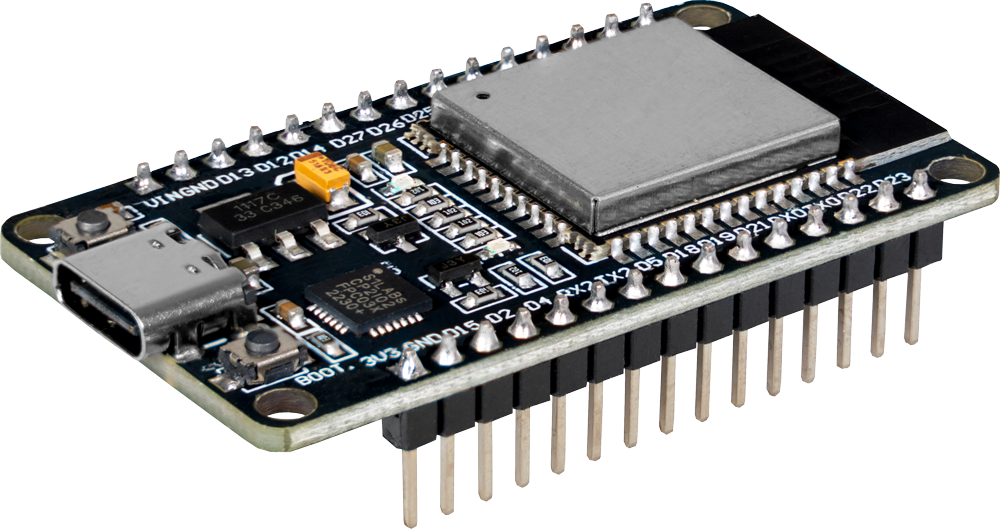
\includegraphics[
            width=1.8cm,
            height=1.1cm,
            keepaspectratio
        ]{images/esp32.png} &
        ESP32 &
        1 &
        Pengendali utama sistem \\

        2 &
        \raisebox{-0.5cm}{%
            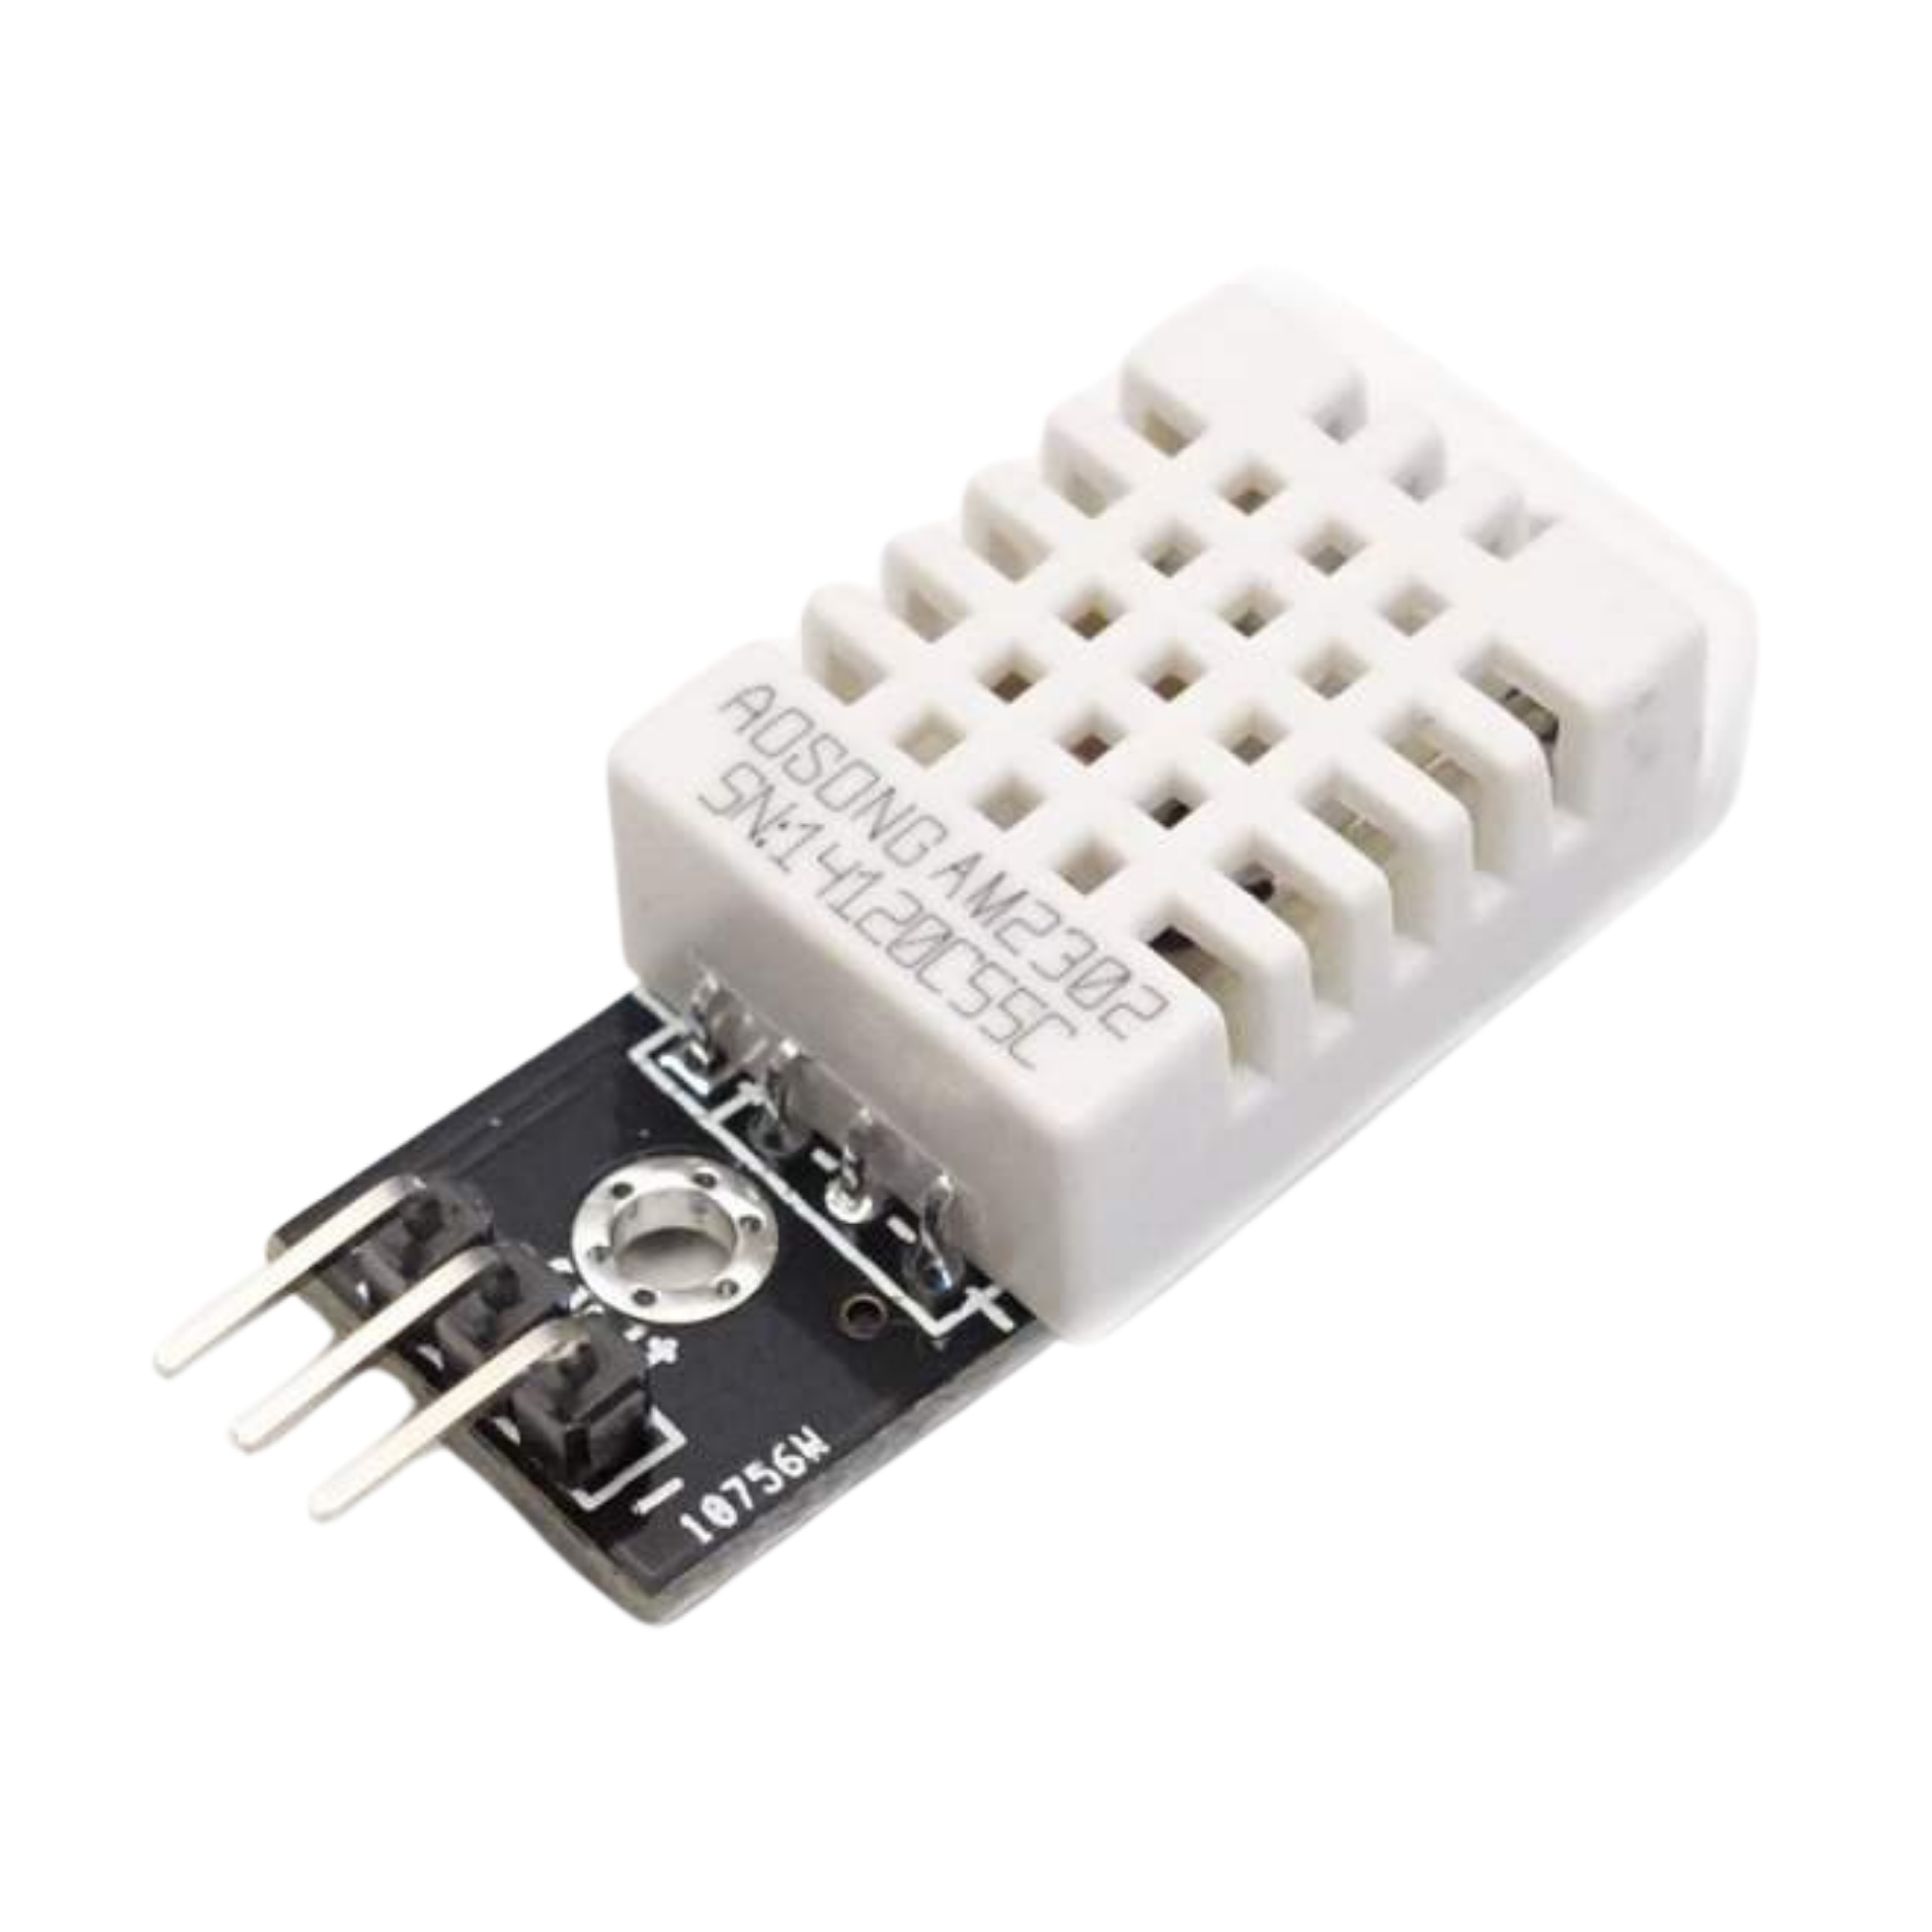
\includegraphics[
                width=1.8cm,
                height=1.1cm,
                keepaspectratio
            ]{images/dht22.png}%
        } &
        DHT22 &
        1 &
        Sensor suhu dan kelembapan udara \\

        3 &
        \raisebox{-0.5cm}{%
            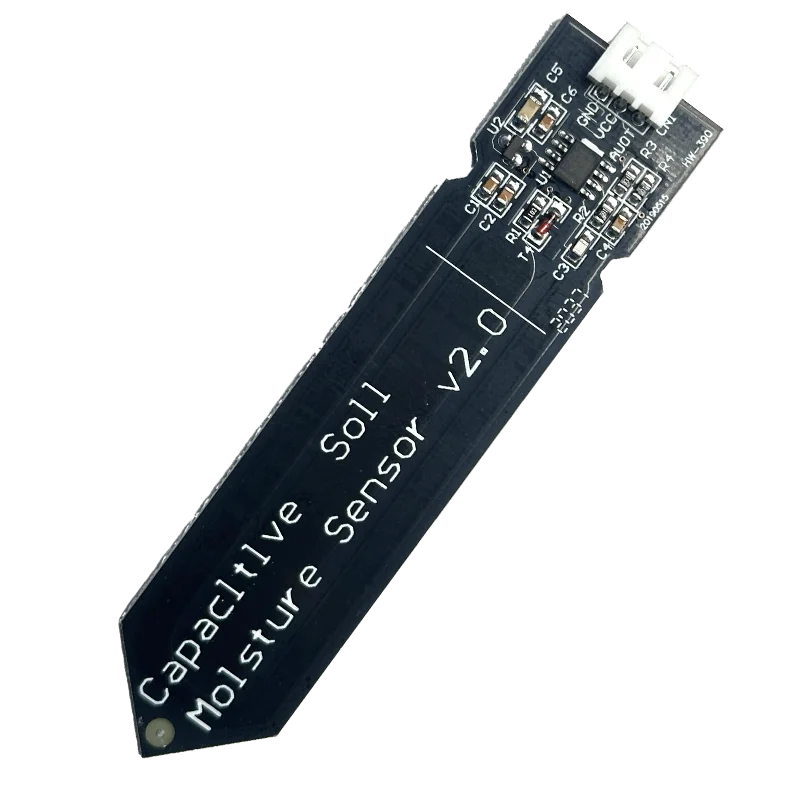
\includegraphics[
                width=1.8cm,
                height=1.1cm,
                keepaspectratio
            ]{images/soil-moisture.png}%
        } &
        Capacitive Soil Moisture Sensor &
        1 &
        Sensor kelembapan tanah/media \\

        4 &
        \multirow{3}{*}{%
            \begin{minipage}[c][3.2cm][c]{2.2cm}
                \centering
                \raisebox{0.5cm}{%
                    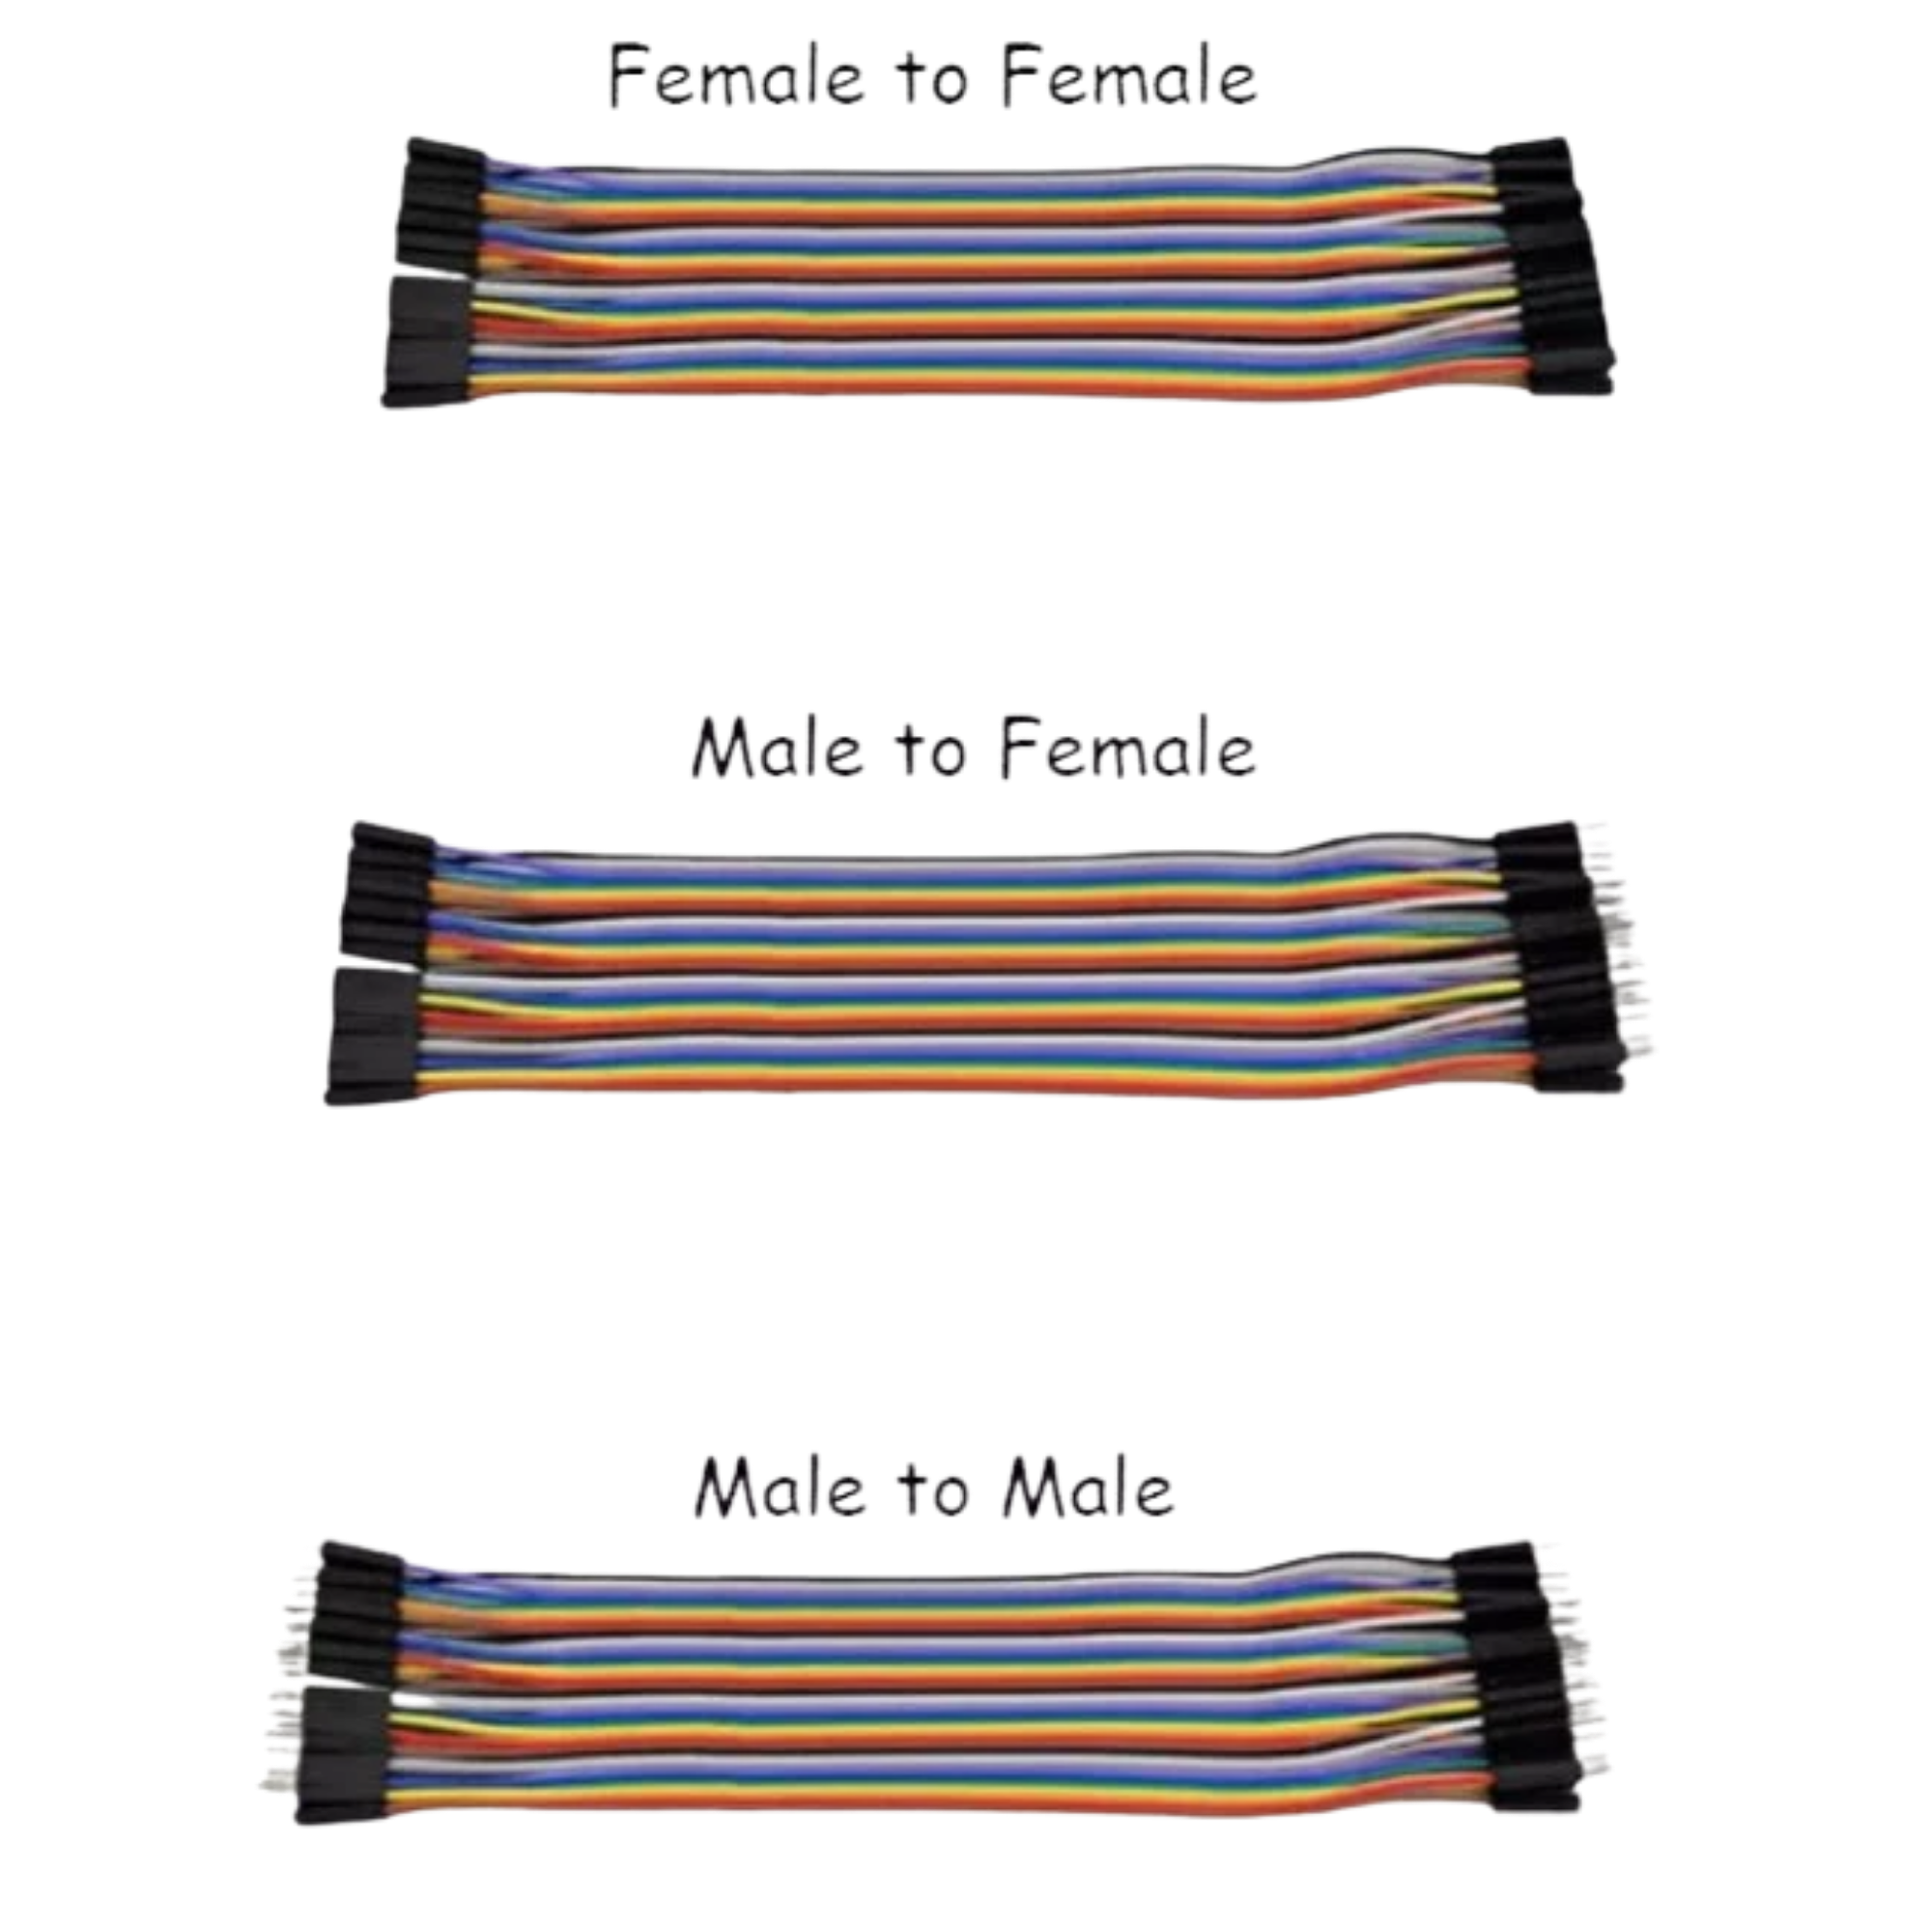
\includegraphics[
                        width=1.8cm,
                        height=2.8cm,
                        keepaspectratio
                    ]{images/kabel-jumper.png}%
                }
            \end{minipage}
        } &
        \rule{0pt}{1cm}
        Kabel jumper F-F &
        Secukupnya &
        Penghubung komponen \\

        & &
        \rule{0pt}{1cm}
        Kabel jumper M-F &
        Secukupnya &
        Penghubung komponen \\

        & &
        \rule{0pt}{1cm}
        Kabel jumper M-M &
        Secukupnya &
        Penghubung komponen \\

        5 &
        \raisebox{-0.5cm}{%
            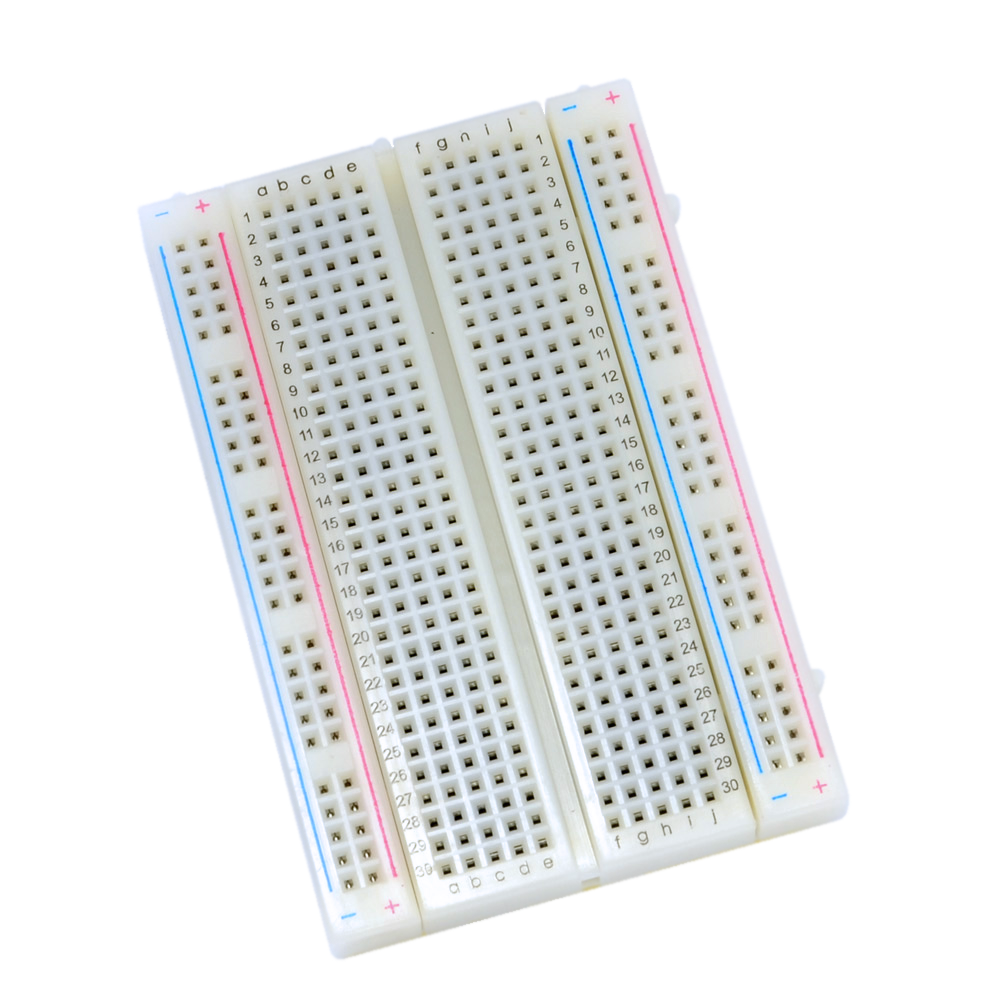
\includegraphics[
                width=1.8cm,
                height=1.1cm,
                keepaspectratio
            ]{images/bread_board.png}%
        } &
        Breadboard &
        1 &
        Media perakitan rangkaian \\

        \bottomrule
    \end{tabularx}
\end{center}

\vspace{0.3cm}

% =========================================================
% TABEL ALAT DAN BAHAN BAGIAN 2
% =========================================================
\begin{center}
    \captionof{table}{Alat dan bahan percobaan (lanjutan)}
    \label{tab:alatbahan2}

    \small
    \renewcommand{\arraystretch}{1.1}

    \begin{tabularx}{\textwidth}{c c L c L}
        \toprule
        \textbf{No.} &
        \textbf{Gambar} &
        \textbf{Alat/Bahan} &
        \textbf{Jumlah} &
        \textbf{Keterangan} \\
        \midrule

        6 &
        \multirow{3}{*}{%
            \begin{minipage}[c][3.2cm][c]{2.2cm}
                \centering
                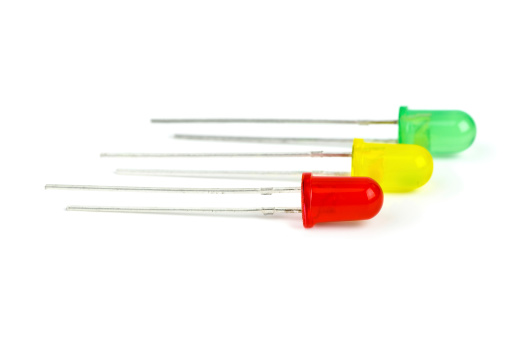
\includegraphics[
                    width=1.8cm,
                    height=2.8cm,
                    keepaspectratio
                ]{images/led.jpg}
            \end{minipage}
        } &
        \rule{0pt}{1cm}
        LED merah &
        1 &
        Indikator kondisi \\

        & &
        \rule{0pt}{1cm}
        LED kuning &
        1 &
        Indikator kondisi \\

        & &
        \rule{0pt}{1cm}
        LED hijau &
        1 &
        Indikator kondisi \\

        7 &
        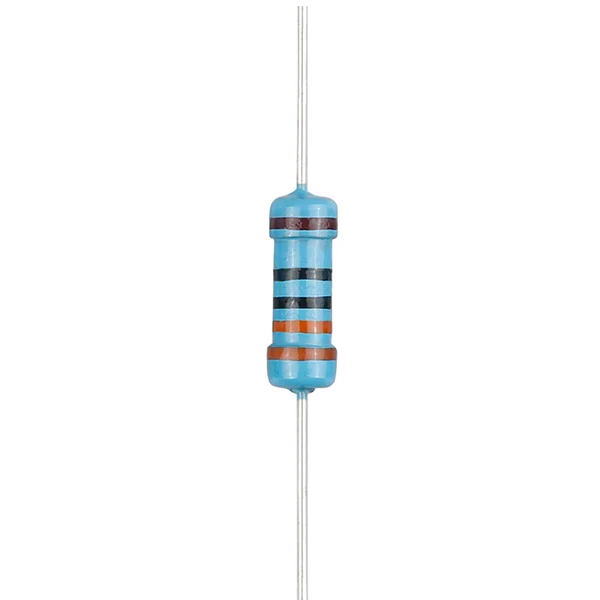
\includegraphics[
            width=1.8cm,
            height=1.1cm,
            keepaspectratio
        ]{images/resistor.png} &
        Resistor $330\,\Omega$ &
        3 &
        Pembatas arus LED \\

        8 &
        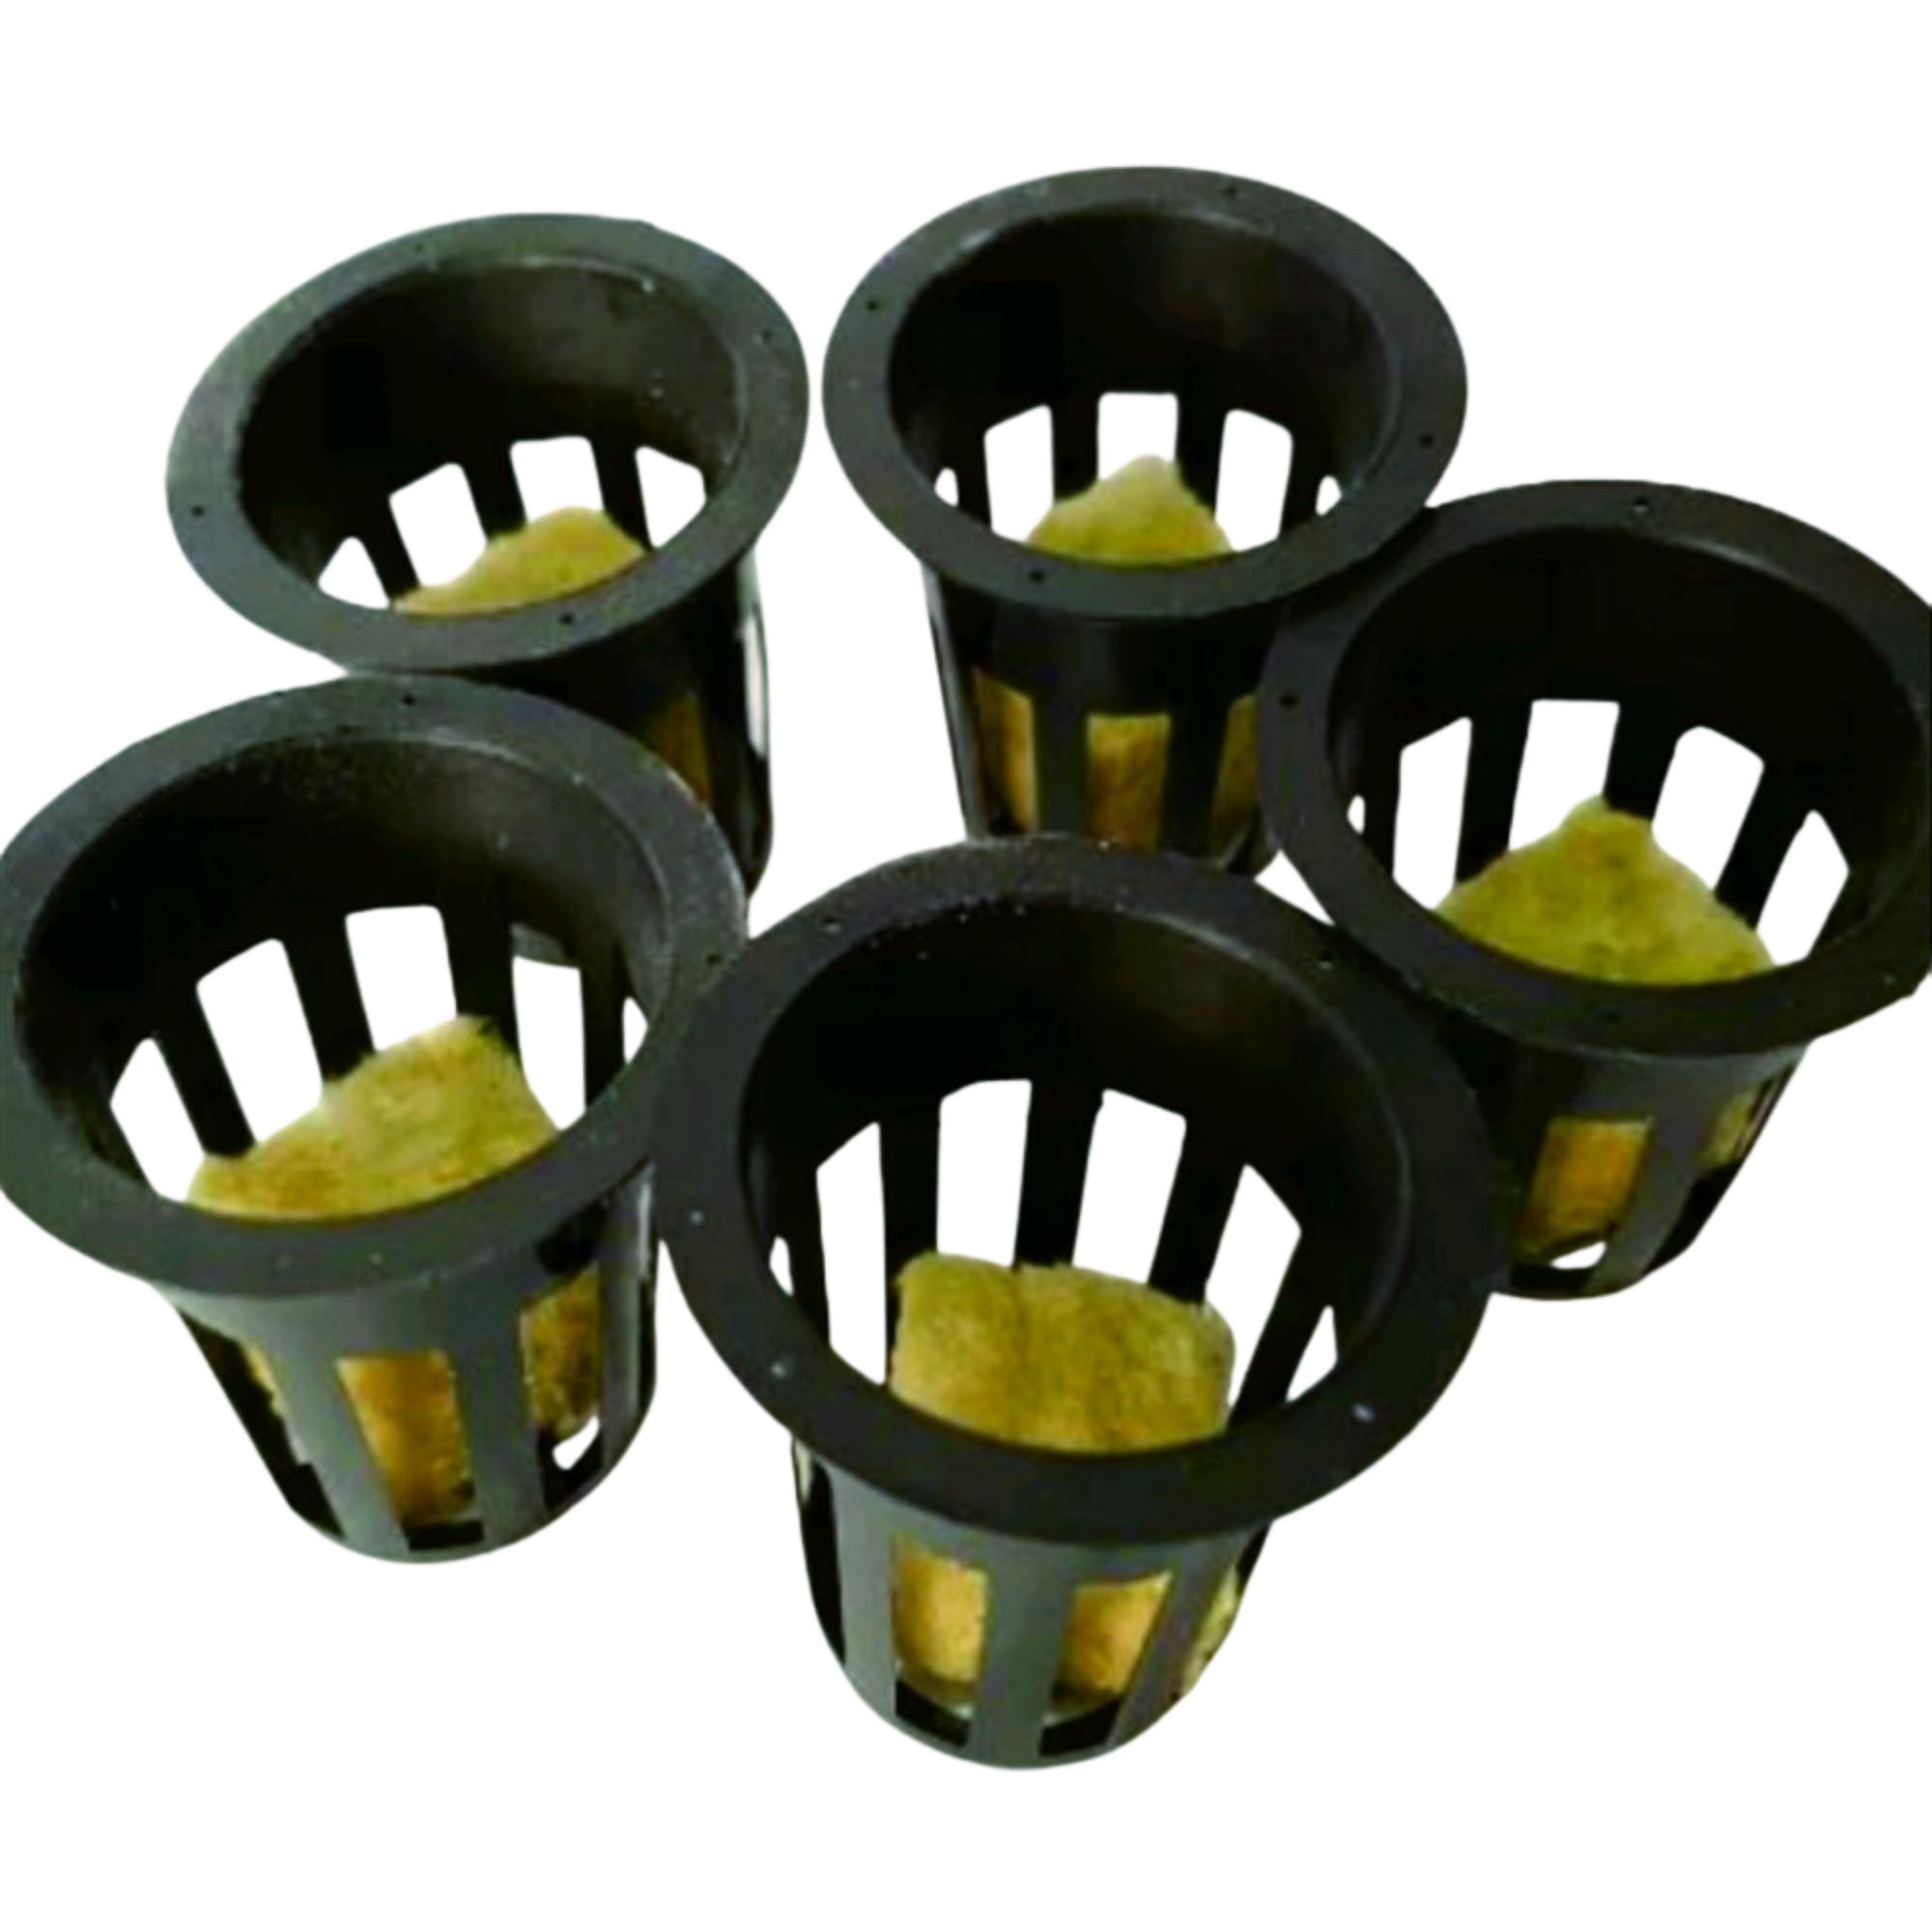
\includegraphics[
            width=1.8cm,
            height=1.1cm,
            keepaspectratio
        ]{images/hidroponik.png} &
        Paket hidroponik &
        1 &
        Objek pengamatan \\

        9 &
        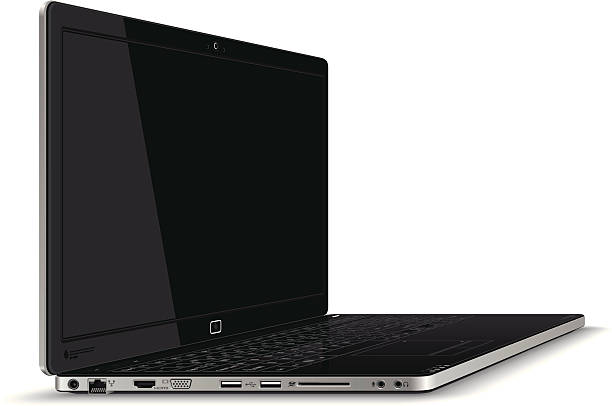
\includegraphics[
            width=1.8cm,
            height=1.1cm,
            keepaspectratio
        ]{images/laptop.jpg} &
        Laptop &
        1 &
        Pemrograman sistem \\

        \bottomrule
    \end{tabularx}
\end{center}

\FloatBarrier

% =========================================================
% 3. DASAR TEORI
% =========================================================
\section{Dasar Teori}

\subsection{Embedded System}

Embedded system adalah sistem komputer yang dibuat khusus untuk menjalankan fungsi tertentu di dalam sebuah perangkat. Sistem ini terdiri dari perangkat keras dan program yang saling bekerja untuk menerima data, mengolahnya, dan menghasilkan keluaran sesuai kebutuhan. Istilah embedded berarti sistem komputer tersebut menjadi bagian dari perangkat dan menjalankan fungsi yang sudah ditentukan. Pada percobaan ini, embedded system digunakan untuk membaca kondisi lingkungan tanaman melalui sensor suhu dan kelembapan tanah, kemudian memberikan indikasi kondisi melalui LED.

Berbeda dengan komputer umum yang dapat digunakan untuk berbagai keperluan, embedded system biasanya dirancang untuk satu atau beberapa fungsi tertentu. Pada percobaan ini, sistem bekerja dengan membaca nilai sensor, mengolah data tersebut, lalu menentukan kondisi tanaman berdasarkan hasil pembacaan.

\subsection{ESP32 sebagai Mikrokontroler}

Mikrokontroler adalah perangkat komputasi dalam satu chip yang memiliki unit pemrosesan, memori, dan antarmuka input-output untuk menjalankan fungsi kendali tertentu. Mikrokontroler dapat membaca masukan dari sensor, menjalankan program yang telah dibuat, dan mengendalikan perangkat keluaran. Kemampuan tersebut membuat mikrokontroler banyak digunakan pada sistem embedded.

ESP32 merupakan mikrokontroler yang digunakan sebagai pengendali utama pada percobaan ini. ESP32 menerima data dari DHT22 dan Capacitive Soil Moisture Sensor, kemudian menjalankan proses pengolahan berdasarkan program yang telah diunggah. Hasil pengolahan selanjutnya digunakan untuk menentukan kondisi LED sebagai keluaran sistem.

\subsection{Sensor}

Sensor adalah komponen yang digunakan untuk mendeteksi suatu besaran fisik dari lingkungan dan mengubahnya menjadi sinyal yang dapat dibaca oleh sistem. Data dari sensor menjadi masukan bagi mikrokontroler untuk menentukan kondisi yang sedang terjadi. Pada percobaan ini digunakan dua sensor dengan fungsi yang berbeda.

DHT22 digunakan untuk membaca suhu dan kelembapan udara. Nilai suhu digunakan sebagai salah satu parameter dalam proses pengambilan keputusan kondisi tanaman. Kelembapan udara dari DHT22 dapat ditampilkan sebagai informasi tambahan, tetapi pada rancangan utama percobaan ini input keputusan difokuskan pada suhu dan kelembapan tanah.

Capacitive Soil Moisture Sensor digunakan untuk mendeteksi tingkat kelembapan pada media tanam. Sensor menghasilkan nilai keluaran yang berubah sesuai kondisi media sehingga dapat digunakan sebagai masukan sistem. Nilai tersebut kemudian dikelompokkan ke dalam kategori seperti kering, lembap, dan basah.

\subsection{Aktuator}

Aktuator adalah komponen yang mengubah sinyal kendali dari sistem menjadi suatu aksi atau keluaran fisik. Dengan kata lain, aktuator merupakan bagian yang melakukan tindakan berdasarkan keputusan yang dihasilkan oleh pengendali. Contoh aktuator dalam kehidupan sehari-hari antara lain lampu yang menyala, kipas yang berputar, atau buzzer yang berbunyi.

Pada percobaan ini, LED digunakan sebagai keluaran indikator sistem. LED tidak melakukan gerakan mekanis seperti motor, tetapi dapat digunakan sebagai aktuator sederhana untuk memberikan respons visual terhadap keputusan sistem. Tiga LED digunakan untuk menunjukkan kondisi yang berbeda, yaitu merah untuk kondisi kurang sesuai, kuning untuk kondisi yang perlu diperhatikan, dan hijau untuk kondisi relatif baik.

\subsection{Konsep Dasar Fuzzy Logic}

\subsubsection{Pengertian Fuzzy Logic}

Fuzzy logic atau logika fuzzy merupakan metode logika yang digunakan untuk merepresentasikan dan mengolah informasi berdasarkan derajat keanggotaan suatu nilai terhadap suatu himpunan. Derajat keanggotaan tersebut dinyatakan dalam bentuk angka pada rentang 0 sampai 1, dengan nilai 0 menunjukkan bahwa suatu nilai sama sekali tidak termasuk dalam himpunan tertentu, sedangkan nilai 1 menunjukkan bahwa suatu nilai sepenuhnya termasuk dalam himpunan tersebut.

Berbanding terbalik dengan fuzzy logic, crisp logic atau logika tegas hanya mengenal dua kondisi, yaitu benar atau salah, sehingga suatu nilai hanya dapat masuk ke dalam satu kategori secara mutlak. Fuzzy logic berbeda dengan crisp logic karena memungkinkan suatu nilai memiliki tingkat keanggotaan terhadap lebih dari satu kategori dalam waktu yang bersamaan. Sebagai contoh, suatu nilai suhu dapat dikatakan sebagian termasuk kategori sedang dan sebagian termasuk kategori panas, tergantung pada seberapa dekat nilai tersebut terhadap batas masing-masing kategori.

Kemampuan tersebut membuat fuzzy logic sesuai digunakan pada sistem yang kondisi lingkungannya tidak selalu memiliki batas yang tegas, seperti sistem pemantauan tanaman yang dibahas pada modul ini. Untuk menentukan derajat keanggotaan, digunakan membership function. Membership function berfungsi untuk menentukan seberapa besar suatu nilai sensor termasuk ke dalam kategori tertentu. Bentuk membership function yang umum digunakan antara lain berbentuk segitiga (triangular) dan trapesium (trapezoidal).

Contoh fungsi keanggotaan segitiga dan trapesium ditunjukkan pada Gambar~\ref{fig:membership-segitiga} dan Gambar~\ref{fig:membership-trapesium}.

\begin{figure}[H]
    \centering
    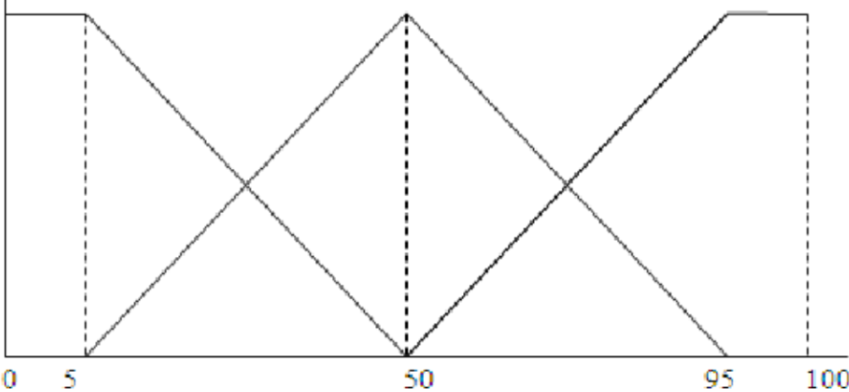
\includegraphics[
        width=0.5\textwidth,
        keepaspectratio
    ]{images/fuzzy-1.png}
    \caption{Contoh membership function segitiga}
    \label{fig:membership-segitiga}
\end{figure}

\begin{figure}[H]
    \centering
    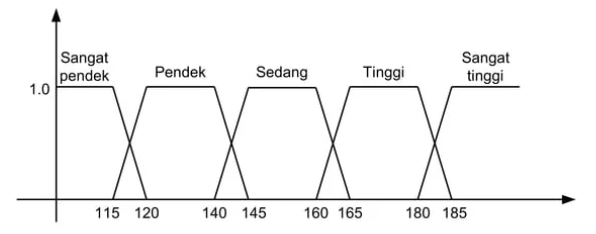
\includegraphics[
        width=0.6\textwidth,
        keepaspectratio
    ]{images/fuzzy-2.png}
    \caption{Contoh membership function trapesium}
    \label{fig:membership-trapesium}
\end{figure}

Pada percobaan ini digunakan membership function berbentuk segitiga. Untuk fungsi segitiga, derajat keanggotaan dapat dihitung menggunakan persamaan berikut.

\[
\mu(x)=
\begin{cases}
0, & x \leq a \\[6pt]
\dfrac{x-a}{b-a}, & a < x \leq b \\[8pt]
\dfrac{c-x}{c-b}, & b < x < c \\[8pt]
0, & x \geq c
\end{cases}
\]

dengan $a$, $b$, dan $c$ merupakan parameter batas yang menentukan bentuk kurva segitiga pada suatu himpunan fuzzy.

\subsubsection{Fuzzy Direct dan Fuzzy PI}

Terdapat dua pendekatan yang umum digunakan dalam penerapan fuzzy logic pada sistem kontrol, yaitu Fuzzy Direct dan Fuzzy PI. Kedua pendekatan tersebut berbeda pada jenis nilai yang digunakan sebagai input fuzzy. Perbedaan tersebut menentukan bagaimana kondisi sistem diproses sebelum menghasilkan keluaran.

Fuzzy Direct merupakan pendekatan yang menggunakan nilai kondisi atau input sistem secara langsung sebagai masukan proses fuzzy, tanpa melalui perhitungan tambahan seperti selisih terhadap suatu nilai acuan. Nilai input yang terbaca oleh sensor langsung diproses melalui tahap fuzzifikasi, penalaran, dan defuzzifikasi untuk menghasilkan output secara langsung. Alur kerja Fuzzy Direct adalah sebagai berikut.

\[
\text{Nilai Sensor}
\rightarrow
\text{Fuzzifikasi}
\rightarrow
\text{Penalaran}
\rightarrow
\text{Defuzzifikasi}
\rightarrow
\text{Keluaran}
\]

Fuzzy PI merupakan pendekatan yang menggunakan error dan perubahan error ($\Delta$ error) sebagai input fuzzy, bukan nilai kondisi sistem secara langsung. Error dihitung sebagai selisih antara kondisi aktual dengan nilai target (setpoint) yang telah ditentukan, sedangkan $\Delta$ error dihitung sebagai selisih antara error saat ini dengan error pada waktu sebelumnya. Pendekatan ini digunakan pada sistem kontrol yang memerlukan penyesuaian keluaran secara bertahap berdasarkan seberapa jauh kondisi aktual menyimpang dari target.

Alur kerja Fuzzy PI adalah sebagai berikut.

\[
\text{Setpoint + Kondisi Aktual}
\rightarrow
\text{Error dan } \Delta\text{ Error}
\rightarrow
\text{Fuzzy PI}
\rightarrow
\text{Perubahan Output Sistem}
\]

Pendekatan yang digunakan pada percobaan ini adalah Fuzzy Direct, karena sistem menggunakan kondisi yang terukur secara langsung sebagai input, yaitu kelembapan tanah dan suhu. Sistem tidak memerlukan perhitungan error terhadap nilai target tertentu, sehingga nilai sensor dapat langsung diproses oleh fuzzy logic. Perubahan suhu atau kelembapan tanah akan langsung memengaruhi keluaran karena perubahan tersebut dapat mengubah derajat keanggotaan dan rule yang aktif.

Fuzzy PI hanya diperkenalkan sebagai pendekatan lain dalam bidang fuzzy control dan tidak diterapkan pada sistem yang dipraktikkan. Pendekatan fuzzy logic yang dikombinasikan dengan pengendali lain seperti PI atau PID juga tidak menjadi bagian dari pembahasan modul ini. Dengan demikian, proses pada percobaan difokuskan pada penggunaan nilai sensor secara langsung untuk menentukan indikator kondisi tanaman melalui LED.

\subsubsection{Metode Inferensi Fuzzy}

Selain dibedakan berdasarkan jenis input yang digunakan, sistem fuzzy logic juga dapat dibedakan berdasarkan metode inferensi yang digunakan pada tahap penalaran dan defuzzifikasi. Beberapa metode inferensi yang umum digunakan antara lain metode Mamdani, metode Sugeno (Takagi-Sugeno-Kang), dan metode Tsukamoto.

Sistem pada modul ini menggunakan keluaran rule berupa nilai crisp tunggal (singleton) untuk setiap kategori, yaitu 0, 50, dan 100, yang kemudian digabungkan langsung menggunakan rata-rata berbobot (weighted average) tanpa melalui proses agregasi himpunan fuzzy maupun perhitungan centroid. Karakteristik tersebut sesuai dengan metode Sugeno orde-nol (zero-order Sugeno), sehingga proses penalaran dan defuzzifikasi pada modul ini mengikuti metode Sugeno.

Metode Mamdani dan Tsukamoto tidak diterapkan pada sistem yang dipraktikkan dan tidak menjadi bagian dari pembahasan modul ini.

\subsubsection{Alur Pengolahan Fuzzy}

Secara umum, proses fuzzy logic pada sistem ini terdiri atas beberapa tahap yang dijalankan secara berurutan, mulai dari pembacaan nilai sensor hingga diperoleh keputusan akhir berupa indikator LED. Tahap tersebut meliputi input, fuzzifikasi, penalaran berdasarkan aturan dasar, defuzzifikasi, hingga output. Setiap tahap memiliki fungsi yang berbeda dalam mengolah data sensor menjadi keputusan sistem.

Alur pengolahan tersebut ditunjukkan pada Gambar~\ref{fig:alur-pengolahan-fuzzy}.

\begin{figure}[H]
    \centering
    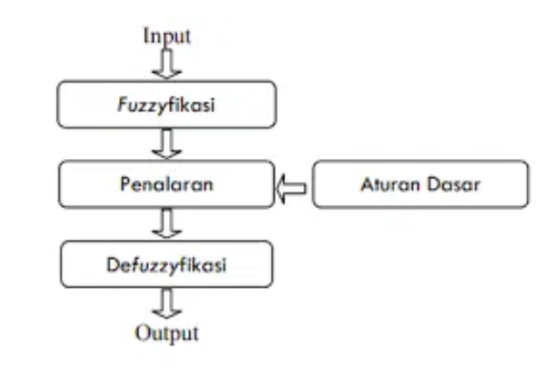
\includegraphics[
        width=0.8\textwidth,
        keepaspectratio
    ]{images/fuzzy-3.png}
    \caption{Alur pengolahan fuzzy}
    \label{fig:alur-pengolahan-fuzzy}
\end{figure}

\textbf{a) Input}

Tahap input merupakan tahap awal dalam proses pengolahan fuzzy. Pada tahap ini, sistem membaca kondisi lingkungan menggunakan sensor DHT22 untuk mengukur suhu dan Capacitive Soil Moisture Sensor untuk mengukur kelembapan tanah. Hasil pembacaan sensor berupa nilai crisp, yaitu nilai dalam bentuk angka yang dapat diukur secara langsung, misalnya suhu sebesar $28^\circ$C dan kelembapan tanah sebesar $32\%$.

Nilai tersebut kemudian digunakan sebagai masukan untuk proses fuzzy pada tahap berikutnya. Pada tahap input, sistem hanya bertugas membaca dan mengambil data dari sensor. Sistem belum menentukan apakah kondisi tanah termasuk kering, lembap, atau basah, maupun apakah suhu termasuk rendah, sedang, atau tinggi.

Hasil pembacaan pada tahap ini menjadi dasar untuk menentukan kondisi tanaman melalui proses fuzzy selanjutnya. Oleh karena itu, semakin baik dan akurat data yang diperoleh sensor, semakin baik pula hasil pengolahan fuzzy yang dihasilkan oleh sistem. Data sensor yang telah terbaca kemudian diteruskan ke tahap fuzzifikasi.

\textbf{b) Fuzzifikasi}

Fuzzifikasi merupakan tahap mengubah nilai input crisp menjadi derajat keanggotaan fuzzy pada masing-masing himpunan yang telah ditentukan. Pada tahap ini, nilai suhu dan kelembapan tanah yang diperoleh dari sensor dimasukkan ke dalam membership function masing-masing variabel untuk mengetahui seberapa besar nilai tersebut termasuk ke dalam kategori tertentu. Bentuk membership function untuk suhu dan kelembapan tanah ditampilkan pada Gambar~\ref{fig:membership-suhu} dan Gambar~\ref{fig:membership-kelembapan}.

\begin{figure}[H]
    \centering
    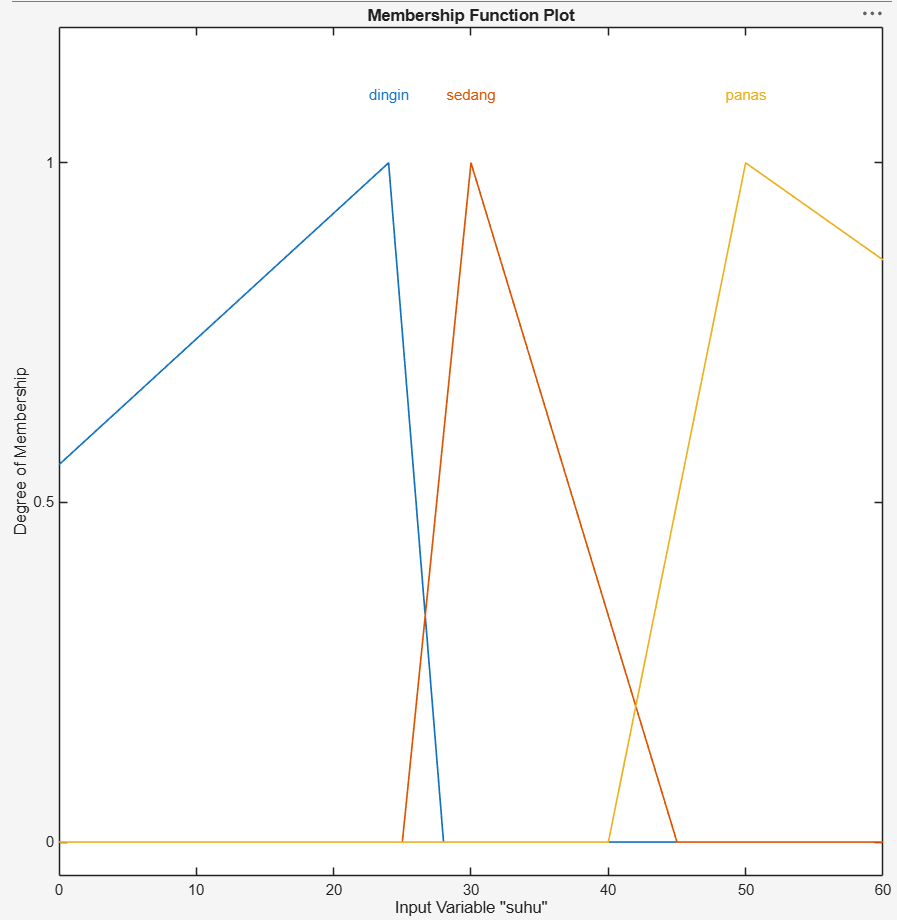
\includegraphics[
        width=0.45\textwidth,
        keepaspectratio
    ]{images/fuzzy-4.png}
    \caption{Membership function suhu}
    \label{fig:membership-suhu}
\end{figure}

\begin{figure}[H]
    \centering
    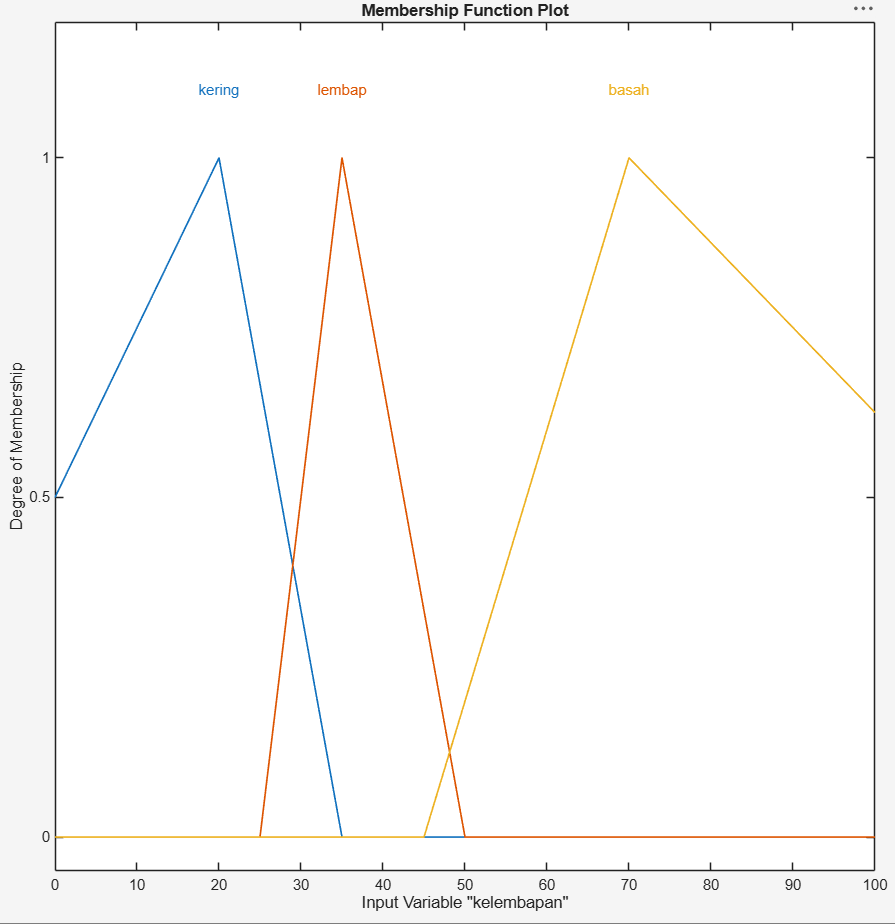
\includegraphics[
        width=0.45\textwidth,
        keepaspectratio
    ]{images/fuzzy-5.png}
    \caption{Membership function kelembapan tanah}
    \label{fig:membership-kelembapan}
\end{figure}

Sebagai contoh, berdasarkan pengujian pada sistem, sensor membaca suhu sebesar $27^\circ$C. Berdasarkan membership function, suhu tersebut termasuk dalam kategori sedang dan panas. Perhitungan derajat keanggotaannya adalah sebagai berikut.

Untuk kategori sedang dengan parameter $[20,25,30]$:

\[
\mu_{\text{sedang}}(27)
=
\frac{30-27}{30-25}
=
\frac{3}{5}
=
0{,}6
\]

Untuk kategori panas dengan parameter $[25,30,35]$:

\[
\mu_{\text{panas}}(27)
=
\frac{27-25}{30-25}
=
\frac{2}{5}
=
0{,}4
\]

Dengan demikian, hasil fuzzifikasi menunjukkan bahwa suhu $27^\circ$C memiliki derajat keanggotaan $0{,}6$ pada kategori sedang dan $0{,}4$ pada kategori panas. Pada saat yang sama, misalkan hasil pembacaan sensor menunjukkan bahwa kelembapan tanah berada sepenuhnya pada kategori lembap, sehingga derajat keanggotaannya pada kategori tersebut adalah $1{,}0$. Nilai $1{,}0$ tersebut menunjukkan tingkat keanggotaan penuh, bukan nilai kelembapan tanah yang sebenarnya.

Hal ini menunjukkan bahwa satu nilai input dapat memiliki derajat keanggotaan pada lebih dari satu kategori secara bersamaan. Dengan kondisi tersebut, terdapat lebih dari satu rule yang dapat aktif pada waktu yang sama. Hasil fuzzifikasi selanjutnya digunakan sebagai input pada tahap penalaran berdasarkan aturan dasar.

\textbf{c) Penalaran Berdasarkan Aturan Dasar}

Penalaran merupakan tahap menentukan hasil berdasarkan hubungan antara input yang telah difuzzifikasi dengan aturan dasar (rule) yang telah disusun sebelumnya. Sistem ini menggunakan rule yang menggabungkan kategori suhu dengan kategori kelembapan tanah menggunakan operator AND. Dalam fuzzy logic, operator AND diselesaikan dengan mengambil nilai minimum dari kedua derajat keanggotaan yang digabungkan.

Setiap rule menghasilkan salah satu kategori keluaran linguistik berupa warna indikator, yaitu hijau atau kuning. Hubungan antara kondisi input dan keluaran tersebut ditentukan melalui rule base sistem fuzzy. Rule base digunakan sebagai dasar untuk menentukan kategori output berdasarkan kombinasi kondisi suhu dan kelembapan tanah.

\begin{figure}[H]
    \centering
    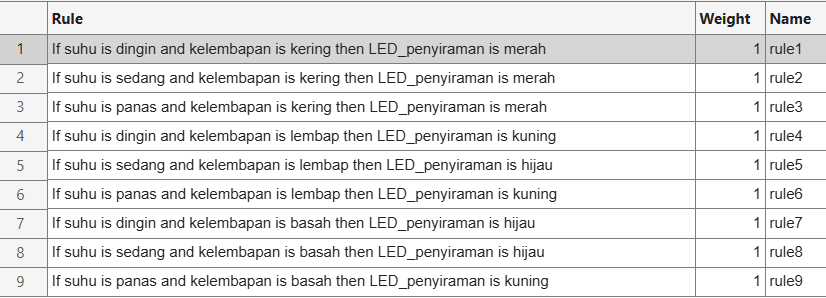
\includegraphics[
        width=0.9\textwidth,
        keepaspectratio
    ]{images/fuzzy-6.png}
    \caption{Rule base sistem fuzzy}
    \label{fig:rule-base-fuzzy}
\end{figure}

Berdasarkan derajat keanggotaan yang telah diperoleh, yaitu suhu sedang sebesar $0{,}6$, suhu panas sebesar $0{,}4$, dan kelembapan tanah lembap sebesar $1{,}0$, maka nilai $\alpha$ untuk setiap rule dihitung sebagai berikut.

Rule 5:

\[
\alpha_5
=
\min(0{,}6;1{,}0)
=
0{,}6
\]

Rule 6:

\[
\alpha_6
=
\min(0{,}4;1{,}0)
=
0{,}4
\]

Rule 5 menggunakan kondisi suhu sedang dan kelembapan lembap sehingga menghasilkan kategori hijau. Rule 6 menggunakan kondisi suhu panas dan kelembapan lembap sehingga menghasilkan kategori kuning. Kedua rule tersebut dapat dihitung karena seluruh derajat keanggotaan yang terlibat bernilai lebih besar dari nol.

Rule yang aktif, yaitu rule dengan $\alpha > 0$, adalah Rule 5 dan Rule 6. Karena masing-masing rule menghasilkan kategori keluaran yang berbeda, yaitu Rule 5 menghasilkan kategori hijau dan Rule 6 menghasilkan kategori kuning, tidak diperlukan proses agregasi dengan nilai maksimum sebagaimana dilakukan apabila terdapat beberapa rule dengan kategori keluaran yang sama. Nilai $\alpha$ masing-masing rule langsung menjadi kekuatan akhir kategori keluarannya.

\[
\alpha_{\text{hijau}} = \alpha_5 = 0{,}6
\]

\[
\alpha_{\text{kuning}} = \alpha_6 = 0{,}4
\]

Nilai-nilai tersebut menunjukkan kekuatan akhir masing-masing kategori keluaran warna indikator setelah mempertimbangkan seluruh rule yang aktif. Hasil penalaran kemudian diteruskan ke tahap defuzzifikasi untuk menghasilkan satu nilai keluaran.

\textbf{d) Defuzzifikasi}

Defuzzifikasi merupakan tahap mengubah hasil penalaran yang masih berbentuk representasi fuzzy menjadi satu nilai crisp atau nilai tunggal yang dapat digunakan oleh sistem. Pada tahap ini, kekuatan masing-masing rule digunakan untuk memperoleh satu nilai keluaran akhir. Proses tersebut dapat digambarkan sebagai berikut.

\[
\text{Hasil Penalaran}
\rightarrow
\text{Nilai Output Crisp}
\]

Metode yang digunakan adalah rata-rata berbobot (weighted average), sesuai dengan metode Sugeno orde-nol, yang menghitung nilai rata-rata dari seluruh rule yang aktif dengan bobot berupa kekuatan masing-masing rule ($\alpha$). Nilai yang dibobotkan berupa nilai crisp tunggal (singleton) dari kategori keluaran rule tersebut, yaitu 0 untuk merah, 50 untuk kuning, dan 100 untuk hijau. Persamaan yang digunakan adalah sebagai berikut.

\[
z=
\frac{\sum_{i=1}^{n}\alpha_i z_i}
{\sum_{i=1}^{n}\alpha_i}
\]

dengan:
\begin{itemize}
    \item $z$ = nilai keluaran akhir,
    \item $\alpha_i$ = kekuatan rule ke-$i$,
    \item $z_i$ = nilai keluaran dari rule ke-$i$.
\end{itemize}

Melanjutkan contoh sebelumnya, Rule 5 menghasilkan keluaran hijau dengan kekuatan $0{,}6$, sedangkan Rule 6 menghasilkan keluaran kuning dengan kekuatan $0{,}4$. Maka nilai keluaran akhir dihitung sebagai berikut.

\begin{align}
z &=
\frac{(0{,}6 \times 100)+(0{,}4 \times 50)}
{0{,}6+0{,}4}
\\[4pt]
&=
\frac{60+20}{1}
\\[4pt]
&= 80
\end{align}

Nilai $80$ merupakan hasil defuzzifikasi atau nilai keluaran akhir sistem. Nilai tersebut kemudian digunakan pada tahap output untuk menentukan warna LED yang akan menyala. Dengan demikian, hasil dari beberapa rule aktif dapat digabungkan menjadi satu nilai keluaran yang dapat digunakan oleh sistem.

\textbf{e) Output}

Nilai crisp ($z$) yang diperoleh dari tahap defuzzifikasi selanjutnya dipetakan ke dalam kategori LED berdasarkan rentang nilai yang telah ditentukan. Pemetaan tersebut digunakan untuk mengubah nilai keluaran menjadi indikator kondisi yang dapat diamati secara langsung oleh pengguna. Rentang kategori LED yang digunakan pada sistem adalah sebagai berikut.

\[
0 \leq z < 25
\quad\rightarrow\quad
\text{LED Merah}
\]

\[
25 \leq z < 75
\quad\rightarrow\quad
\text{LED Kuning}
\]

\[
75 \leq z \leq 100
\quad\rightarrow\quad
\text{LED Hijau}
\]

Melanjutkan contoh sebelumnya, nilai $z=80$ berada pada rentang $75 \leq z \leq 100$, sehingga sistem menghasilkan LED hijau. Dengan demikian, output yang diterima oleh pengguna sistem bukan berupa angka mentah, melainkan indikasi kondisi tanaman secara langsung melalui LED. Hal tersebut memungkinkan perubahan kondisi suhu dan kelembapan tanah diamati melalui perubahan indikator warna yang dihasilkan sistem.

% =========================================================
% 4. PERSIAPAN PERCOBAAN
% =========================================================
\section{Persiapan Percobaan}

Sebelum memulai percobaan, pastikan laptop, perangkat lunak, dan komponen yang digunakan telah siap. Ikuti konfigurasi berikut sebelum melakukan perakitan dan pengunggahan program.

\subsection{Persiapan Perangkat Lunak}

Perangkat lunak yang digunakan dalam percobaan adalah Arduino IDE. Arduino IDE digunakan untuk menulis program, memilih board ESP32, memilih port komunikasi, mengunggah program ke mikrokontroler, dan memantau data melalui Serial Monitor.

Pastikan Arduino IDE telah terpasang pada laptop sebelum percobaan dimulai. Gunakan versi terbaru yang dapat diunduh melalui situs resmi Arduino pada tautan berikut:

\url{https://www.arduino.cc/en/software/}

\begin{enumerate}
    \item Buka situs resmi Arduino dan unduh Arduino IDE sesuai dengan sistem operasi yang digunakan.
    \item Pasang Arduino IDE pada laptop.
    \item Buka Arduino IDE dan pastikan program dapat dijalankan.
\end{enumerate}

\subsection{Board Package dan Library}

Program membutuhkan board package dan library agar Arduino IDE dapat mengenali perangkat dan menjalankan fungsi sensor. Board package digunakan agar Arduino IDE dapat melakukan proses kompilasi dan pengunggahan program ke ESP32. Library digunakan untuk menyediakan fungsi komunikasi dan pembacaan sensor yang diperlukan oleh program.

\begin{enumerate}
    \item Buka Arduino IDE.
    \item Masuk ke \textbf{File} $\rightarrow$ \textbf{Preferences}.
    \item Pada bagian \textbf{Additional Boards Manager URLs}, tambahkan URL berikut:

    \url{https://espressif.github.io/arduino-esp32/package_esp32_index.json}

    \item Buka \textbf{Tools} $\rightarrow$ \textbf{Board} $\rightarrow$ \textbf{Boards Manager}.
    \item Cari \textbf{esp32} dan pasang \textbf{esp32 by Espressif Systems}.
    \item Setelah proses instalasi selesai, pilih \textbf{ESP32 Dev Module} melalui \textbf{Tools} $\rightarrow$ \textbf{Board}.
    \item Hubungkan ESP32 ke laptop menggunakan kabel USB.
    \item Pilih port komunikasi ESP32 melalui \textbf{Tools} $\rightarrow$ \textbf{Port}.
\end{enumerate}

Library yang dibutuhkan dalam percobaan dapat dipasang melalui Arduino IDE. Buka \textbf{Tools} $\rightarrow$ \textbf{Manage Libraries}. Pada kolom pencarian, masukkan nama library yang dibutuhkan, kemudian pilih library yang sesuai dan klik \textbf{Install}. Library yang digunakan dalam percobaan dirangkum pada Tabel~\ref{tab:library}.

\begin{table}[H]
    \centering
    \caption{Library yang digunakan}
    \label{tab:library}
    \begin{tabularx}{\textwidth}{c L L}
        \toprule
        \textbf{No.} &
        \textbf{Library} &
        \textbf{Fungsi} \\
        \midrule

        1 &
        DHT Sensor Library &
        Membaca data suhu dan kelembapan dari sensor DHT22 \\

        2 &
        Adafruit Unified Sensor &
        Library pendukung yang dibutuhkan oleh DHT Sensor Library \\

        \bottomrule
    \end{tabularx}
\end{table}

Pastikan seluruh library yang dibutuhkan telah berhasil terpasang sebelum program diunggah ke ESP32.

% =========================================================
% 5. PERANCANGAN SISTEM
% =========================================================
\section{Perancangan Sistem}

\begin{figure}[H]
    \centering
    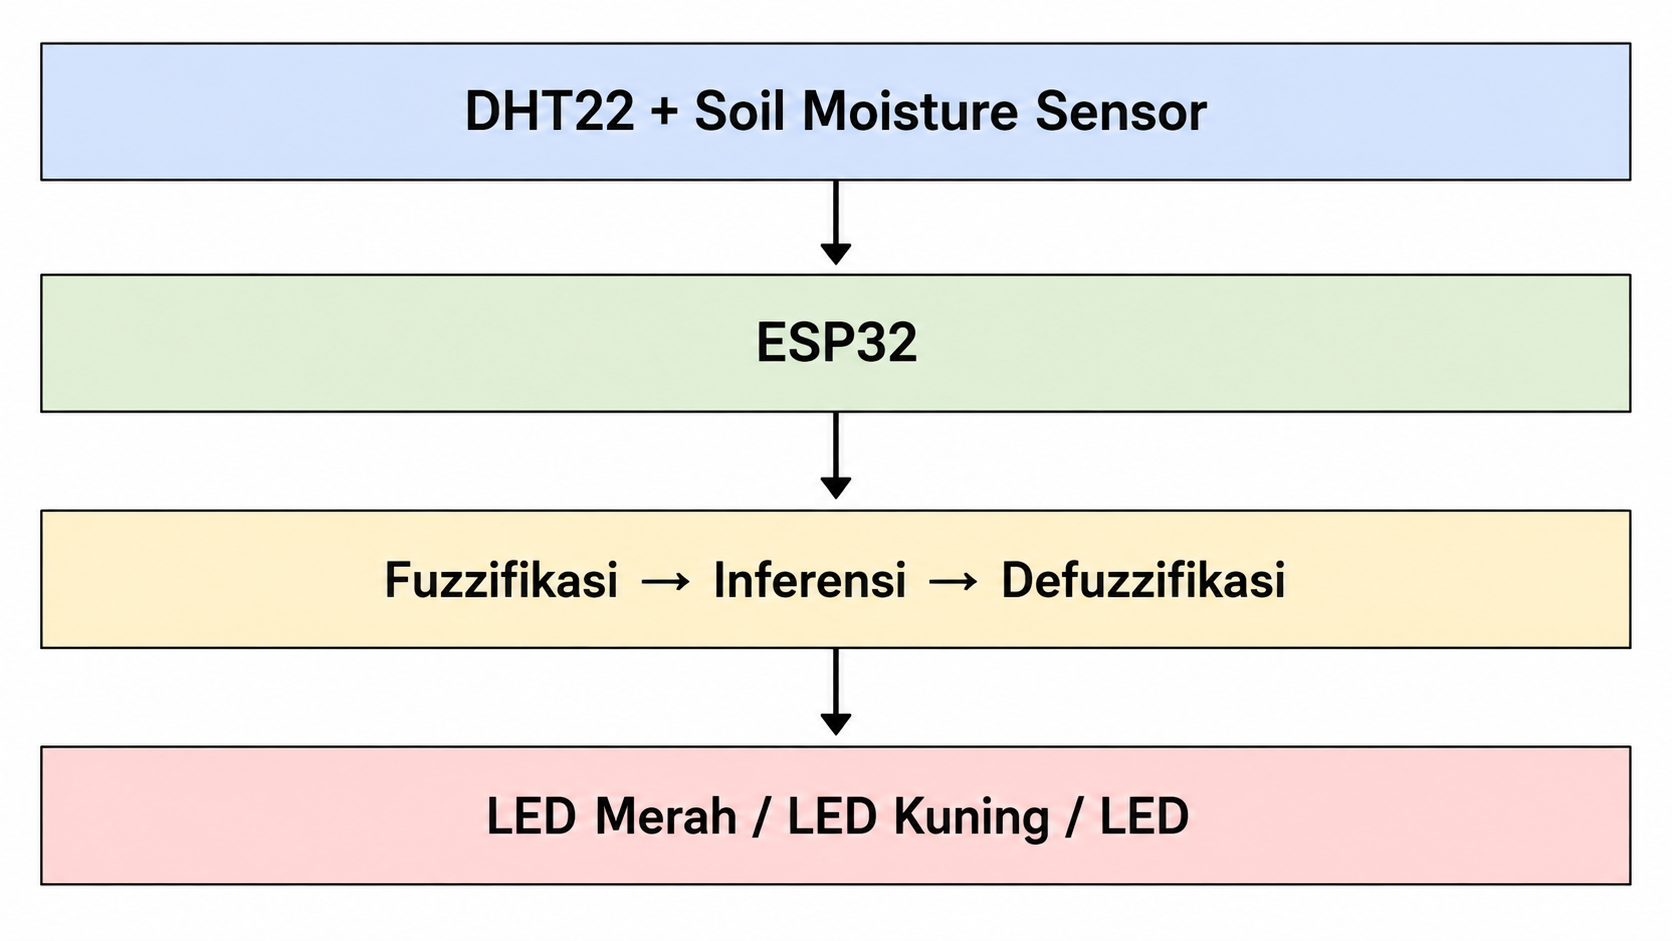
\includegraphics[
        width=0.6\textwidth
    ]{images/diagram-blok-sistem.png}
    \caption{Diagram blok sistem percobaan}
    \label{fig:blok-sistem}
\end{figure}

Alur kerja sistem ditunjukkan pada Gambar~\ref{fig:blok-sistem}. Sistem dimulai dari pembacaan data suhu dan kelembapan tanah oleh sensor. Data dari sensor kemudian diterima dan dibaca oleh ESP32, dengan nilai dari sensor analog dibaca menggunakan Analog to Digital Converter (ADC). Selanjutnya, data yang diperoleh diproses menggunakan logika fuzzy untuk menentukan kondisi sistem berdasarkan aturan yang telah dirancang. Hasil pengolahan tersebut kemudian digunakan untuk menentukan LED yang menyala sesuai dengan kondisi sistem.

\subsection{Perancangan Input dan Output}

Dua variabel digunakan sebagai masukan sistem, yaitu suhu dan kelembapan media. Kategori input dan maknanya dirangkum pada Tabel~\ref{tab:kategoriinput}. Masing-masing variabel dibagi menjadi tiga kategori untuk menyederhanakan proses pengambilan keputusan dan penyusunan rule. Setiap kategori memiliki batas nilai yang telah ditentukan sesuai dengan parameter membership function yang digunakan pada sistem.

\begin{table}[H]
    \centering
    \caption{Kategori input sistem}
    \label{tab:kategoriinput}
    \begin{tabularx}{\textwidth}{p{0.25\textwidth} p{0.15\textwidth} X}
        \toprule
        \textbf{Variabel} &
        \textbf{Himpunan} &
        \textbf{Makna} \\
        \midrule

        Suhu &
        Dingin &
        Suhu relatif rendah untuk kondisi pengamatan \\

        Suhu &
        Sedang &
        Suhu berada pada rentang kondisi sedang untuk pengamatan \\

        Suhu &
        Panas &
        Suhu relatif tinggi untuk kondisi pengamatan \\

        Kelembapan media &
        Kering &
        Media tanam memiliki tingkat kelembapan rendah \\

        Kelembapan media &
        Lembap &
        Media tanam memiliki tingkat kelembapan sedang \\

        Kelembapan media &
        Basah &
        Media tanam memiliki tingkat kelembapan tinggi \\

        \bottomrule
    \end{tabularx}
\end{table}

Output sistem terdiri dari tiga kategori yang dirangkum pada Tabel~\ref{tab:output} dan digunakan untuk merepresentasikan hasil keputusan fuzzy. Nilai keluaran dari proses defuzzifikasi kemudian dipetakan ke kategori LED yang telah ditentukan, sehingga hasil keputusan dapat ditampilkan secara langsung.

\begin{table}[H]
    \centering
    \caption{Kategori output sistem}
    \label{tab:output}
    \begin{tabularx}{\textwidth}{c c c X}
        \toprule
        \textbf{Kategori} &
        \textbf{LED} &
        \textbf{Nilai Output} &
        \textbf{Makna} \\
        \midrule

        1 &
        Merah &
        0 &
        Kondisi kurang sesuai \\

        2 &
        Kuning &
        50 &
        Kondisi perlu diperhatikan \\

        3 &
        Hijau &
        100 &
        Kondisi relatif baik \\

        \bottomrule
    \end{tabularx}
\end{table}

\subsection{Membership Function}

Membership function digunakan untuk mengubah nilai sensor menjadi derajat keanggotaan. Parameter fungsi keanggotaan yang digunakan pada sistem dirangkum pada Tabel~\ref{tab:mf}. Parameter tersebut digunakan langsung oleh ESP32 pada proses fuzzifikasi sebelum dilanjutkan ke tahap inferensi.

\begin{table}[H]
    \centering
    \caption{Parameter membership function}
    \label{tab:mf}
    \small
    \begin{tabularx}{\textwidth}{l l c c c X}
        \toprule
        \textbf{Variabel} &
        \textbf{Himpunan} &
        \textbf{a} &
        \textbf{b} &
        \textbf{c} &
        \textbf{Keterangan} \\
        \midrule

        Suhu & Dingin &
        24 &
        24 &
        28 &
        Fungsi keanggotaan suhu dingin \\

        Suhu & Sedang &
        25 &
        30 &
        45 &
        Fungsi keanggotaan suhu sedang \\

        Suhu & Panas &
        40 &
        50 &
        60 &
        Fungsi keanggotaan suhu panas \\

        \addlinespace
        Kelembapan media & Kering &
        20 &
        20 &
        35 &
        Fungsi keanggotaan kelembapan kering \\

        Kelembapan media & Lembap &
        25 &
        35 &
        50 &
        Fungsi keanggotaan kelembapan lembap \\

        Kelembapan media & Basah &
        45 &
        70 &
        70 &
        Fungsi keanggotaan kelembapan basah \\

        \bottomrule
    \end{tabularx}
\end{table}

Penguji tidak perlu menghitung seluruh kombinasi membership function secara manual. Parameter membership function telah dimasukkan ke dalam program, sehingga ESP32 melakukan proses fuzzifikasi berdasarkan nilai suhu dan kelembapan tanah yang terbaca oleh sensor.

\subsection{Fuzzy Rule}

Rule base pada Tabel~\ref{tab:fuzzy-rule} dibuat dengan mengombinasikan tiga kondisi suhu dan tiga kondisi kelembapan media. Setiap kombinasi input menghasilkan salah satu dari tiga keluaran fuzzy, yaitu buruk, sedang, atau baik. Keluaran fuzzy tersebut kemudian digunakan dalam proses inferensi dan defuzzifikasi untuk memperoleh nilai output akhir yang digunakan dalam menentukan LED.

\begin{table}[H]
    \centering
    \caption{Rule base fuzzy}
    \label{tab:fuzzy-rule}
    \small
    \renewcommand{\arraystretch}{1.15}

    \begin{tabularx}{\textwidth}{c c c c c X}
        \toprule
        \textbf{Rule} &
        \textbf{Suhu} &
        \textbf{Kelembapan} &
        \textbf{Output Fuzzy} &
        \textbf{Nilai} &
        \textbf{LED} \\
        \midrule

        R1 &
        Dingin &
        Kering &
        Buruk &
        0 &
        Merah \\

        R2 &
        Dingin &
        Lembap &
        Sedang &
        50 &
        Kuning \\

        R3 &
        Dingin &
        Basah &
        Baik &
        100 &
        Hijau \\

        R4 &
        Sedang &
        Kering &
        Buruk &
        0 &
        Merah \\

        R5 &
        Sedang &
        Lembap &
        Baik &
        100 &
        Hijau \\

        R6 &
        Sedang &
        Basah &
        Baik &
        100 &
        Hijau \\

        R7 &
        Panas &
        Kering &
        Buruk &
        0 &
        Merah \\

        R8 &
        Panas &
        Lembap &
        Sedang &
        50 &
        Kuning \\

        R9 &
        Panas &
        Basah &
        Sedang &
        50 &
        Kuning \\

        \bottomrule
    \end{tabularx}
\end{table}

Setiap rule menggunakan operator AND untuk menggabungkan kondisi suhu dan kelembapan media. Susunan hubungan antara kondisi input dan keluaran ditampilkan pada Gambar~\ref{fig:rule-base-fuzzy}. Kekuatan setiap rule ditentukan menggunakan nilai minimum dari derajat keanggotaan kedua input. Misalnya, jika derajat keanggotaan suhu sedang adalah 0,6 dan derajat keanggotaan kelembapan lembap adalah 0,8, maka kekuatan rule yang menggabungkan kedua kondisi tersebut adalah 0,6.

Rule R1, R4, dan R7 menghasilkan output buruk dengan nilai representatif 0 sehingga diarahkan ke LED merah. Rule R2 dan R8 menghasilkan output sedang dengan nilai representatif 50 sehingga diarahkan ke LED kuning. Sementara itu, rule R3, R5, dan R6 menghasilkan output baik dengan nilai representatif 100 sehingga diarahkan ke LED hijau. Rule R9 menghasilkan output sedang dengan nilai representatif 50 karena kondisi suhu panas tetap perlu diperhatikan meskipun kelembapan media berada pada kategori basah.

Nilai output pada tabel merupakan nilai representatif (singleton) yang digunakan dalam proses defuzzifikasi. Nilai tersebut belum menjadi hasil akhir sistem karena beberapa rule dapat aktif secara bersamaan. Hasil akhir diperoleh dengan menggabungkan kekuatan rule yang aktif menggunakan metode rata-rata berbobot (Sugeno).

\clearpage

Nilai akhir kemudian dipetakan ke indikator LED berdasarkan rentang berikut:

\[
\begin{aligned}
0 &\leq z < 25 &&\rightarrow \text{LED Merah} \\
25 &\leq z < 75 &&\rightarrow \text{LED Kuning} \\
75 &\leq z \leq 100 &&\rightarrow \text{LED Hijau}
\end{aligned}
\]

% =========================================================
% 6. PERCOBAAN 1
% =========================================================
\section{Percobaan 1: Pembacaan Kondisi Lingkungan}

Percobaan pertama dilakukan untuk memastikan bahwa sensor dapat digunakan sebagai sumber data sistem. Penguji mengamati nilai suhu dan kelembapan tanah sebelum proses pengambilan keputusan diaktifkan. Pada percobaan ini, perubahan kelembapan media dibuat menggunakan beberapa kondisi rockwool, sedangkan perubahan suhu diamati pada kondisi suhu ruangan, saat sensor terkena aliran udara dingin, dan saat sensor terkena aliran udara panas.

\subsection{Prosedur Percobaan}

\begin{enumerate}
    \item Siapkan ESP32, DHT22, Capacitive Soil Moisture Sensor, breadboard, kabel jumper, rockwool, dan sumber udara dengan kondisi suhu yang berbeda.
    \item Rangkai DHT22 dan Capacitive Soil Moisture Sensor sesuai konfigurasi yang digunakan.
    \item Hubungkan ESP32 ke laptop.
    \item Buka program pembacaan sensor.
    \item Sesuaikan nomor pin pada program dengan wiring aktual.
    \item Unggah program ke ESP32.
    \item Buka Serial Monitor dan pastikan data sensor dapat terbaca.
    \item Lakukan pengamatan pada beberapa kondisi media dengan tingkat kelembapan yang berbeda.
    \item Catat nilai kelembapan media yang terbaca pada setiap kondisi.
    \item Amati pembacaan suhu pada kondisi lingkungan yang berbeda.
    \item Catat nilai suhu yang terbaca pada setiap kondisi.
    \item Bandingkan hasil pembacaan sensor pada seluruh kondisi pengamatan.
    \item Catat seluruh hasil pengamatan.
\end{enumerate}

\begin{lstlisting}[language=C++, caption={Program pembacaan sensor untuk Percobaan 1}, label={lst:percobaan1}]
#include <DHT.h>

#define SOIL_PIN 34

#define DHT_PIN 4
#define DHT_TYPE DHT22

DHT dht(DHT_PIN, DHT_TYPE);

const int SOIL_DRY_RAW = 3000;
const int SOIL_WET_RAW = 1200;

void setup()
{
  Serial.begin(115200);
  dht.begin();
}

void loop()
{
  float temperature = dht.readTemperature();

  int raw = analogRead(SOIL_PIN);

  float soilPercent =
    ((float)(SOIL_DRY_RAW - raw) /
     (SOIL_DRY_RAW - SOIL_WET_RAW)) * 100.0;

  soilPercent = constrain(soilPercent, 0, 100);

  Serial.print("Suhu: ");
  Serial.print(temperature, 1);
  Serial.println(" C");

  Serial.print("Kelembapan Tanah: ");
  Serial.print(soilPercent, 1);
  Serial.println(" %");

  Serial.println("--------------------");

  delay(2000);
}
\end{lstlisting}

Rangkaian sensor pada Percobaan 1 ditunjukkan pada Gambar~\ref{fig:wiring-percobaan1}.

\begin{figure}[H]
    \centering
    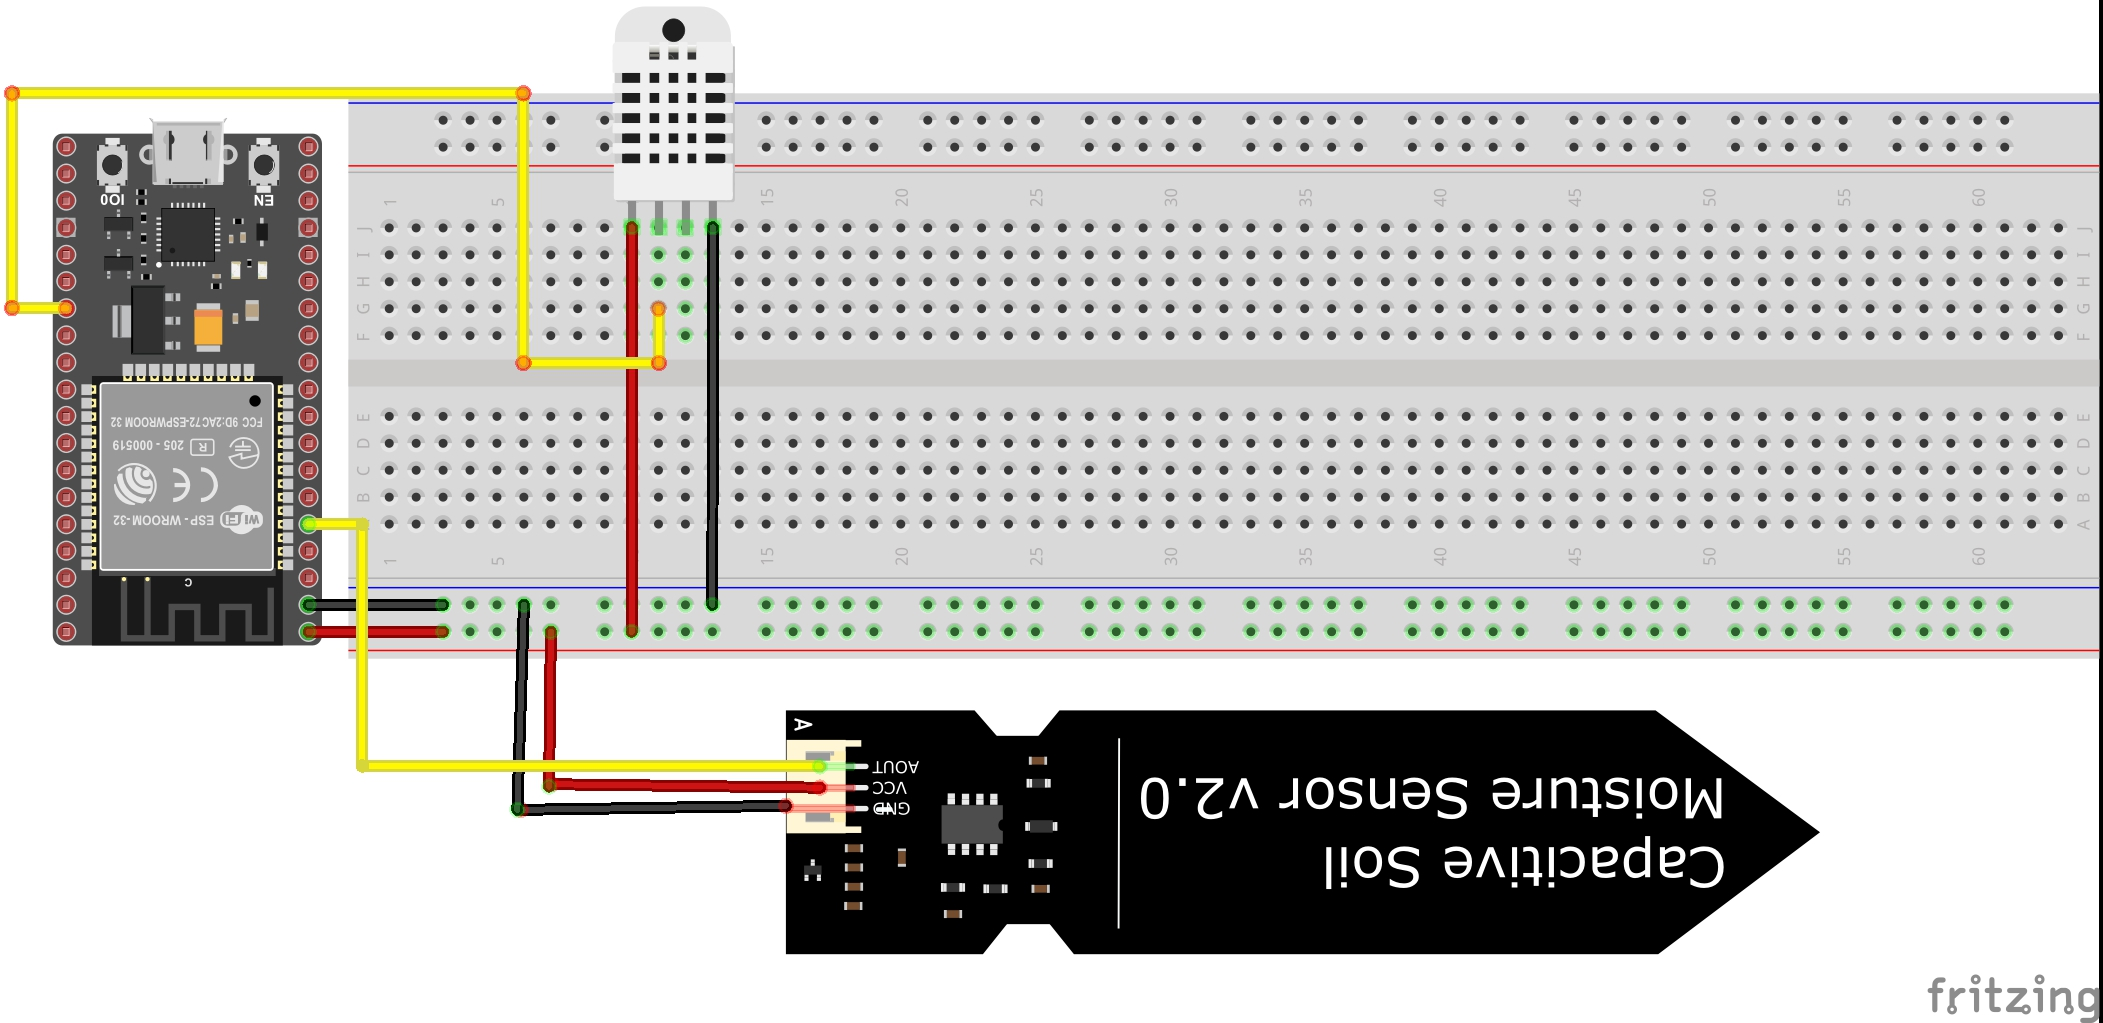
\includegraphics[
        width=0.85\textwidth,
        keepaspectratio
    ]{images/percobaan_1.jpg}
    \caption{Wiring sensor DHT22 dan Capacitive Soil Moisture Sensor pada Percobaan 1}
    \label{fig:wiring-percobaan1}
\end{figure}

\subsection{Analisis Percobaan}

Analisis dilakukan dengan membandingkan pembacaan sensor pada kondisi rockwool yang berbeda dan pada beberapa kondisi suhu. Perhatikan perubahan nilai kelembapan tanah ketika rockwool berada pada kondisi kering, lembap, dan basah. Selain itu, amati perbedaan suhu yang terbaca pada kondisi suhu ruangan, ketika sensor terkena aliran udara dingin, dan ketika sensor terkena aliran udara panas.

\subsubsection*{Target Pengamatan}

\begin{itemize}
    \item[$\checkbox$] Data suhu dapat terbaca pada Serial Monitor.
    \item[$\checkbox$] Data kelembapan tanah dapat terbaca.
    \item[$\checkbox$] Nilai sensor kelembapan berubah pada setiap kondisi rockwool.
    \item[$\checkbox$] Nilai suhu berubah ketika sensor berada di kondisi suhu berbeda.
    \item[$\checkbox$] Pembacaan sensor dapat digunakan sebagai input sistem.
    \item[$\checkbox$] Tidak terdapat pembacaan sensor yang tidak wajar selama pengamatan.
\end{itemize}

\subsubsection*{Catatan}

\noindent
\makebox[\textwidth]{\hrulefill}

\vspace{0.4cm}

\noindent
\makebox[\textwidth]{\hrulefill}

\vspace{0.4cm}

\noindent
\makebox[\textwidth]{\hrulefill}

% =========================================================
% 7. PERCOBAAN 2
% =========================================================
\section{Percobaan 2: Implementasi Metode Pengambilan Keputusan}

Percobaan kedua menggabungkan pembacaan sensor dengan proses pengambilan keputusan. Nilai sensor digunakan sebagai input untuk membership function dan rule yang telah dirancang. Hasil pengolahan ditampilkan melalui LED agar perubahan keputusan dapat diamati secara langsung pada beberapa kombinasi kondisi kelembapan media dan suhu yang berbeda.

\subsection{Prosedur Percobaan}

\begin{enumerate}
    \item Lanjutkan dari rangkaian Percobaan 1.
    \item Pastikan seluruh koneksi sensor masih terpasang dengan benar.
    \item Tambahkan tiga LED sebagai indikator keluaran.
    \item Pasang resistor LED sesuai kebutuhan rangkaian.
    \item Masukkan parameter membership function ke dalam program.
    \item Masukkan rule base ke dalam program.
    \item Unggah program ke ESP32.
    \item Buka Serial Monitor dan pastikan data suhu, kelembapan media, output, dan status LED dapat terbaca.
    \item Lakukan pengujian menggunakan beberapa kondisi media dengan tingkat kelembapan yang berbeda.
    \item Lakukan pengujian pada beberapa kondisi suhu yang berbeda.
    \item Catat nilai suhu, kelembapan media, output, dan LED pada setiap kondisi pengujian.
    \item Bandingkan perubahan output dan LED terhadap perubahan kondisi input.
    \item Bandingkan hasil pengamatan dengan rule base yang telah dirancang.
    \item Catat seluruh hasil pengamatan.
\end{enumerate}

\begin{lstlisting}[language=C++, caption={Program implementasi fuzzy logic untuk Percobaan 2}, label={lst:percobaan2}]
#include <DHT.h>

#define SOIL_PIN 34

#define DHT_PIN 4
#define DHT_TYPE DHT22

#define LED_MERAH_PIN 25
#define LED_KUNING_PIN 26
#define LED_HIJAU_PIN 27

DHT dht(DHT_PIN, DHT_TYPE);

const int SOIL_DRY_RAW = 3000;
const int SOIL_WET_RAW = 1200;


float suhuDingin(float x)
{
  if (x <= 24) return 1.0;
  if (x >= 28) return 0.0;

  return (28.0 - x) / (28.0 - 24.0);
}

float suhuSedang(float x)
{
  if (x <= 25 || x >= 45) return 0.0;
  if (x == 30) return 1.0;

  if (x < 30)
    return (x - 25.0) / (30.0 - 25.0);

  return (45.0 - x) / (45.0 - 30.0);
}

float suhuPanas(float x)
{
  if (x <= 40) return 0.0;
    if (x >= 60) return 0.0;
    if (x <= 50)
        return (x - 40.0) / (50.0 - 40.0);

    return (60.0 - x) / (60.0 - 50.0);
}


float tanahKering(float x)
{
  if (x <= 20) return 1.0;
  if (x >= 35) return 0.0;

  return (35.0 - x) / (35.0 - 20.0);
}

float tanahLembap(float x)
{
  if (x <= 25 || x >= 50) return 0.0;
  if (x == 35) return 1.0;

  if (x < 35)
    return (x - 25.0) / (35.0 - 25.0);

  return (50.0 - x) / (50.0 - 35.0);
}

float tanahBasah(float x)
{
  if (x <= 45) return 0.0;
  if (x >= 70) return 1.0;
  return (x - 45.0) / (70.0 - 45.0);
}


void setLED(int ledPin)
{
  digitalWrite(LED_MERAH_PIN, LOW);
  digitalWrite(LED_KUNING_PIN, LOW);
  digitalWrite(LED_HIJAU_PIN, LOW);

  digitalWrite(ledPin, HIGH);
}


void setup()
{
  Serial.begin(115200);

  dht.begin();

  pinMode(LED_MERAH_PIN, OUTPUT);
  pinMode(LED_KUNING_PIN, OUTPUT);
  pinMode(LED_HIJAU_PIN, OUTPUT);

  digitalWrite(LED_MERAH_PIN, LOW);
  digitalWrite(LED_KUNING_PIN, LOW);
  digitalWrite(LED_HIJAU_PIN, LOW);
}


void loop()
{
  float temperature = dht.readTemperature();

  int rawSoil = analogRead(SOIL_PIN);

  float soilPercent =
    ((float)(SOIL_DRY_RAW - rawSoil) /
     (SOIL_DRY_RAW - SOIL_WET_RAW)) * 100.0;

  soilPercent = constrain(soilPercent, 0, 100);

  if (isnan(temperature))
  {
    Serial.println("Gagal membaca DHT22");
    delay(2000);
    return;
  }


  float dingin = suhuDingin(temperature);
    float sedang = suhuSedang(temperature);
  float panas  = suhuPanas(temperature);

  float kering = tanahKering(soilPercent);
  float lembap = tanahLembap(soilPercent);
  float basah  = tanahBasah(soilPercent);

  
  float r1 = min(dingin, kering);
  float r2 = min(dingin, lembap);
  float r3 = min(dingin, basah);

    float r4 = min(sedang, kering);
    float r5 = min(sedang, lembap);
    float r6 = min(sedang, basah);

  float r7 = min(panas, kering);
  float r8 = min(panas, lembap);
  float r9 = min(panas, basah);


  float numerator =
      (r1 * 0)   +
      (r2 * 50)  +
      (r3 * 100) +
      (r4 * 0)   +
      (r5 * 100) +
      (r6 * 100) +
      (r7 * 0)   +
      (r8 * 50)  +
      (r9 * 50);

  float denominator =
      r1 + r2 + r3 +
      r4 + r5 + r6 +
      r7 + r8 + r9;

  float output = 0;

  if (denominator > 0)
  {
    output = numerator / denominator;
  }


  String ledStatus;

  if (output >= 75)
  {
    setLED(LED_HIJAU_PIN);
    ledStatus = "HIJAU";
  }
  else if (output >= 25)
  {
    setLED(LED_KUNING_PIN);
    ledStatus = "KUNING";
  }
  else
  {
    setLED(LED_MERAH_PIN);
    ledStatus = "MERAH";
  }


  Serial.print("Suhu: ");
  Serial.print(temperature, 1);
  Serial.println(" C");

  Serial.print("Kelembapan Tanah: ");
  Serial.print(soilPercent, 1);
  Serial.println(" %");

  Serial.print("Output: ");
  Serial.println(output, 1);

  Serial.print("LED: ");
  Serial.println(ledStatus);

  Serial.println("--------------------");

  delay(2000);
}
\end{lstlisting}

Rangkaian lengkap pada Percobaan 2 ditunjukkan pada Gambar~\ref{fig:wiring-percobaan2}.

\begin{figure}[H]
    \centering
    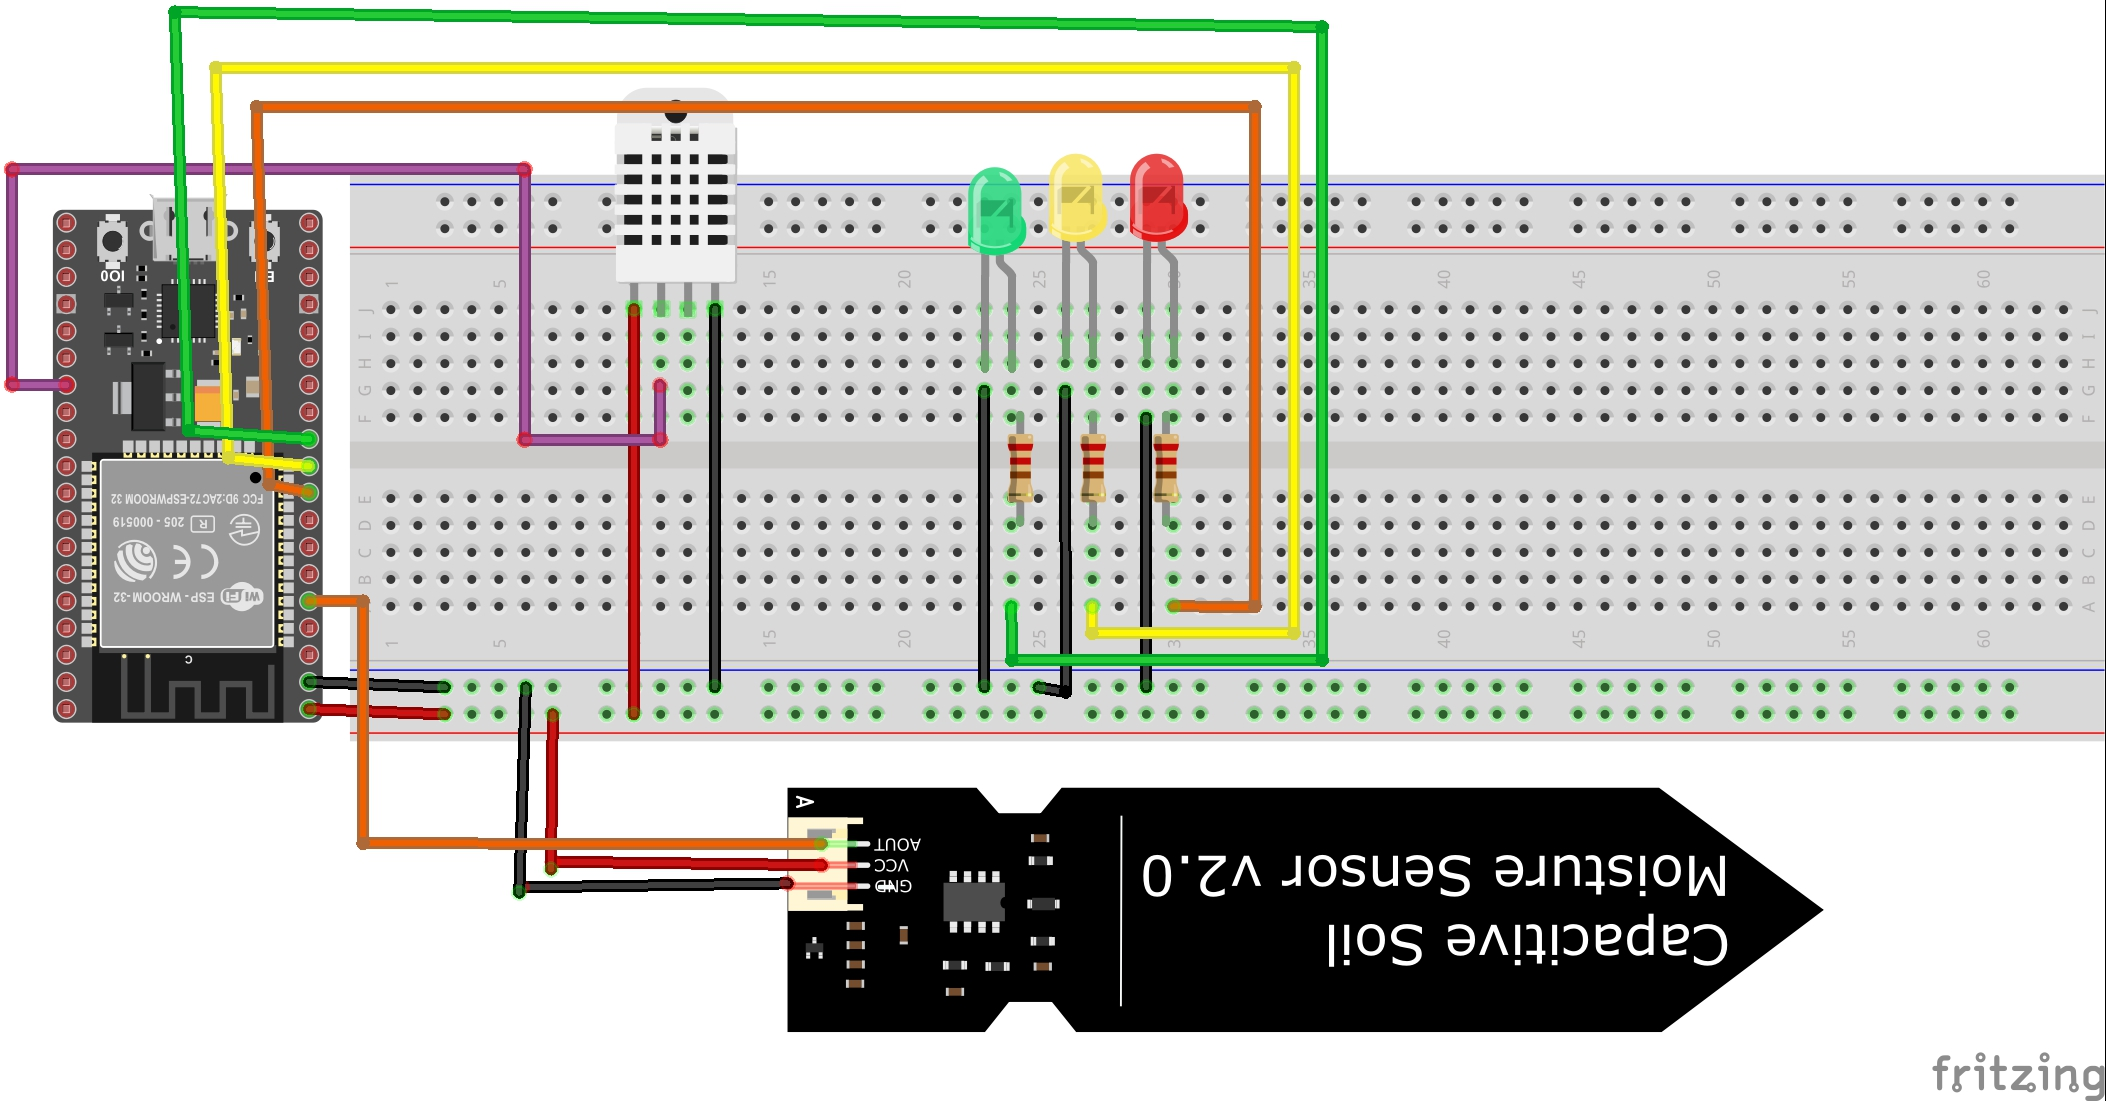
\includegraphics[
        width=0.85\textwidth,
        keepaspectratio
    ]{images/percobaan_2.jpg}
    \caption{Wiring lengkap ESP32, DHT22, Capacitive Soil Moisture Sensor, dan LED pada Percobaan 2}
    \label{fig:wiring-percobaan2}
\end{figure}

\subsection{Tabel Pengamatan}

\begin{table}[H]
    \centering
    \caption{Tabel pengamatan kondisi lingkungan}
    \label{tab:pengamatan}
    \small

    \begin{tabularx}{\textwidth}{c L c c c c L}
        \toprule
        \textbf{No.} &
        \textbf{Kondisi} &
        \textbf{Suhu} &
        \textbf{Kelembapan Tanah} &
        \textbf{Prediksi} &
        \textbf{LED Aktual} &
        \textbf{Catatan} \\
        \midrule

        1 &
        Suhu ruangan + rockwool kering &
        & & & & \\

        2 &
        Suhu ruangan + rockwool lembap &
        & & & & \\

        3 &
        Suhu ruangan + rockwool basah &
        & & & & \\

        4 &
        Udara dingin + rockwool kering &
        & & & & \\

        5 &
        Udara dingin + rockwool lembap &
        & & & & \\

        \bottomrule
    \end{tabularx}
\end{table}

\begin{table}[H]
    \centering
    \caption{Tabel pengamatan kondisi lingkungan (lanjutan)}
    \label{tab:pengamatan-lanjutan}
    \small

    \begin{tabularx}{\textwidth}{c L c c c c L}
        \toprule
        \textbf{No.} &
        \textbf{Kondisi} &
        \textbf{Suhu} &
        \textbf{Kelembapan Tanah} &
        \textbf{Prediksi} &
        \textbf{LED Aktual} &
        \textbf{Catatan} \\
        \midrule

        6 &
        Udara dingin + rockwool basah &
        & & & & \\

        7 &
        Udara panas + rockwool kering &
        & & & & \\

        8 &
        Udara panas + rockwool lembap &
        & & & & \\

        9 &
        Udara panas + rockwool basah &
        & & & & \\

        \bottomrule
    \end{tabularx}
\end{table}

Nilai pada Tabel~\ref{tab:pengamatan} dan Tabel~\ref{tab:pengamatan-lanjutan} harus diisi berdasarkan hasil pengukuran langsung selama percobaan. Jangan menggunakan nilai pada contoh perhitungan sebagai data pengamatan. Catatan harus menunjukkan kondisi yang benar-benar terlihat pada saat sistem dijalankan.

\subsection{Analisis Percobaan}

Analisis pada percobaan kedua berfokus pada hubungan antara perubahan input dan keluaran sistem. Perhatikan perubahan LED pada berbagai kondisi rockwool serta perubahan keluaran ketika suhu berubah akibat aliran udara dingin dan aliran udara panas. Hasil pengamatan dibandingkan dengan kecenderungan yang dihasilkan oleh membership function dan rule yang telah dibuat.

\subsubsection*{Target Pengamatan}

\begin{itemize}
    \item[$\checkbox$] Nilai sensor dapat diproses menggunakan membership function.
    \item[$\checkbox$] Rule dapat digunakan untuk menghasilkan keluaran.
    \item[$\checkbox$] Sistem dapat membaca kondisi rockwool yang berbeda.
    \item[$\checkbox$] Perubahan kelembapan rockwool memengaruhi hasil pengolahan.
    \item[$\checkbox$] Perubahan suhu memengaruhi hasil pengolahan.
    \item[$\checkbox$] Output berubah mengikuti perubahan kondisi input.
    \item[$\checkbox$] LED menyala sesuai dengan hasil pengolahan.
    \item[$\checkbox$] Hasil aktual mengikuti kecenderungan yang diprediksi.
    \item[$\checkbox$] Sistem tidak menghasilkan kondisi output yang tidak didefinisikan.
\end{itemize}

\subsubsection*{Catatan}

\noindent
\makebox[\textwidth]{\hrulefill}

\vspace{0.4cm}

\noindent
\makebox[\textwidth]{\hrulefill}

\vspace{0.4cm}

\noindent
\makebox[\textwidth]{\hrulefill}

% =========================================================
% 8. EVALUASI PERCOBAAN
% =========================================================
\section{Evaluasi Percobaan}

Evaluasi dilakukan untuk mengetahui apakah sistem telah bekerja sesuai dengan rancangan yang dibuat. Penguji membandingkan hasil pembacaan sensor, hasil pengolahan fuzzy, dan LED yang menyala pada setiap kondisi pengujian. Hasil evaluasi digunakan untuk melihat kesesuaian antara kondisi input, keluaran sistem, dan rule yang telah dirancang.

\subsection*{Pertanyaan Evaluasi}

\begin{enumerate}
    \item Berdasarkan Tabel~\ref{tab:pengamatan} dan Tabel~\ref{tab:pengamatan-lanjutan}, kombinasi suhu dan kelembapan tanah apa yang menghasilkan LED hijau, kuning, dan merah? Jelaskan hubungannya dengan rule base pada Tabel~\ref{tab:fuzzy-rule}.

    \item Bandingkan hasil sistem pada kondisi suhu ruangan, udara dingin, dan udara panas. Jelaskan bagaimana perubahan suhu memengaruhi nilai output dan LED yang dihasilkan.

    \item Apakah hasil LED aktual sesuai dengan prediksi berdasarkan rule? Jika terdapat perbedaan, jelaskan kemungkinan penyebabnya berdasarkan hasil pembacaan sensor.
\end{enumerate}

\subsection*{Kesimpulan Pengamatan}

\noindent
\makebox[\textwidth]{\hrulefill}

\vspace{0.4cm}

\noindent
\makebox[\textwidth]{\hrulefill}

\vspace{0.4cm}

\noindent
\makebox[\textwidth]{\hrulefill}

% =========================================================
% 9. PENUTUP
% =========================================================
\section{Penutup}

Pada percobaan ini, penguji telah menggunakan data suhu dan kelembapan tanah sebagai input sistem monitoring kondisi tanaman. Data sensor diproses menggunakan membership function dan rule sederhana untuk menghasilkan keputusan yang kemudian ditampilkan melalui LED. Rangkaian tersebut menunjukkan bagaimana metode pengambilan keputusan dapat diimplementasikan secara langsung pada ESP32 sebagai platform embedded system.

Melalui dua percobaan, penguji mengamati pembacaan sensor, proses pengolahan fuzzy, dan respons sistem terhadap berbagai kombinasi kondisi suhu dan kelembapan tanah. Hasil pengamatan digunakan untuk membandingkan kondisi input dengan keluaran yang dihasilkan oleh sistem serta melihat kesesuaian antara hasil aktual dan rule yang telah dirancang. Evaluasi pada akhir percobaan membantu penguji memahami hubungan antara perubahan input, proses fuzzy, dan keputusan yang ditampilkan melalui LED.

\end{document}